\documentclass{buthesis}

\usepackage{hologo}
\usepackage{booktabs}
\usepackage{float} 
\usepackage{hyphenat}
\usepackage{tabularx,array}
\usepackage{amsmath}
\usepackage{svg,graphicx}
\usepackage{tabularx, ragged2e}
\newcolumntype{Y}{>{\RaggedRight\arraybackslash}X}
\usepackage[utf8]{inputenc}
\usepackage{newunicodechar}
\usepackage[nottoc]{tocbibind}
\usepackage[titletoc]{appendix}
\setcounter{tocdepth}{2}
\usepackage{listings}
\usepackage{xcolor}
\usepackage[utf8]{inputenc}
\usepackage{listings}
\usepackage{listingsutf8}
\usepackage{import}
\usepackage[ruled,vlined]{algorithm2e}

\svgsetup{
	inkscapeexe={C:/Program Files/Inkscape/bin/inkscape.exe},
	inkscapelatex=true,
	inkscapearea=page
}


\lstset{
  inputencoding=utf8,
  basicstyle=\ttfamily\small,
  breaklines=true,
  literate=
    {–}{{-}}1 {—}{{---}}1 {…}{{\ldots}}1
    {→}{{$\to$}}1 {←}{{$\leftarrow$}}1 {⇒}{{$\Rightarrow$}}1
    {α}{{$\alpha$}}1 {β}{{$\beta$}}1 {γ}{{$\gamma$}}1 {δ}{{$\delta$}}1
    {π}{{$\pi$}}1 {σ}{{$\sigma$}}1 {τ}{{$\tau$}}1
    {Δ}{{$\Delta$}}1 {Σ}{{$\Sigma$}}1 {Ω}{{$\Omega$}}1
}

\lstset{
  basicstyle=\ttfamily\small,
  breaklines=true,
  breakatwhitespace=true,
  columns=fullflexible,
  keepspaces=true,
  tabsize=2,
  frame=single,
  rulecolor=\color{black!20},
  xleftmargin=0.5em, xrightmargin=0.5em,
  aboveskip=0.75\baselineskip, belowskip=0.75\baselineskip,
  postbreak=\mbox{\textellipsis\space}
}


\newunicodechar{π}{\ensuremath{\pi}}
\newunicodechar{α}{\ensuremath{\alpha}}
\newunicodechar{β}{\ensuremath{\beta}}
\newunicodechar{γ}{\ensuremath{\gamma}}
\newunicodechar{δ}{\ensuremath{\delta}}
\newunicodechar{ε}{\ensuremath{\varepsilon}}
\newunicodechar{θ}{\ensuremath{\theta}}
\newunicodechar{λ}{\ensuremath{\lambda}}
\newunicodechar{μ}{\ensuremath{\mu}}
\newunicodechar{ρ}{\ensuremath{\rho}}
\newunicodechar{σ}{\ensuremath{\sigma}}
\newunicodechar{τ}{\ensuremath{\tau}}
\newunicodechar{φ}{\ensuremath{\varphi}}
\newunicodechar{ω}{\ensuremath{\omega}}
\newunicodechar{Δ}{\ensuremath{\Delta}}
\newunicodechar{Λ}{\ensuremath{\Lambda}}
\newunicodechar{Σ}{\ensuremath{\Sigma}}
\newunicodechar{Ω}{\ensuremath{\Omega}}



\begin{document}

\title{Detecting Interprocedural Software Vulnerabilities Using Causal Deep Learning}
\author{Md Iqbal Hossain Shuvo}

\beforepreface
\prefacesection{Abstract}


Software vulnerabilities in large systems rarely stem from a single line of code. Instead, they emerge from chains of decisions and data flows that cross multiple functions, files, and modules. Existing tools, including both traditional static and dynamic analysis and modern learning-based detectors, are good at flagging suspicious locations but rarely explain how a vulnerability actually arises and propagates through a program. As a result, their predictions are often brittle, difficult to trust, and only weakly connected to the steps a developer must take to fix the underlying problem.
	
This thesis addresses this limitation by treating the entire path from the initial cause of a vulnerability to its exploitable endpoint as the main object of analysis. The central goal is to reconstruct \emph{executable interprocedural root-to-sink vulnerability chains} that a developer can follow across functions and files. To achieve this, the work first builds a program representation that records how control and data move within and between functions in real software projects. On top of this representation, a learning-based model is trained not only to decide whether a piece of code is vulnerable, but also to identify and assemble the sequence of steps that carry the vulnerable state from its origin to a sensitive operation.
	
Beyond simply producing these chains, the thesis introduces criteria to check whether the explanations are truly aligned with the model’s behaviour. These criteria probe how predictions change when key parts of a chain are edited and measure how much of the model’s attention falls on the reconstructed path. An empirical study on real-world repositories shows that focusing on interprocedural chains leads to more stable predictions, clearer explanations, and guidance that is better suited to debugging and remediation than conventional “black-box” scores. In this way, the thesis moves vulnerability detection closer to tools that do not just say \emph{where} a problem is, but explain \emph{how} and \emph{why} it can be exploited.





\prefacesection{Acknowledgments}

I would like to express my sincere gratitude to everyone who contributed to the successful completion of this thesis. First, I thank my Supervisor, Y M, for their unwavering support, invaluable guidance, and patience throughout this research journey.

\figurespagetrue
\tablespagetrue

\afterpreface

\chapter{Introduction}
\label{chap:intro}

Software vulnerability detection remains a critical yet complex challenge in software engineering. Modern digital infrastructure, financial services, scientific workflows, and everyday communication all depend on large, evolving software systems. As these systems scale in size and heterogeneity, contemporary codebases span millions of lines of code and are developed by distributed teams over long periods of time. This growth in complexity increases architectural coupling and the likelihood that subtle defects persist into production. When such defects are exploitable, they become security vulnerabilities that threaten confidentiality, integrity, and availability, and their effects may propagate across dependent components and services~\cite{Li2022Empirical,yang2022natural,Le2024MBU}.

Traditional vulnerability detection techniques provide important, but incomplete, coverage of this problem space. \emph{Static analysis} examines code without executing it, relying on rule-based systems, type reasoning, data-flow frameworks, and abstract interpretation to infer program behaviour at scale~\cite{Allix2024,Ruiz2023,taviss2024asm2seq}. \emph{Dynamic analysis} executes programs with concrete or instrumented inputs to observe runtime behaviour directly, often using monitoring, tracing, or sandboxing to detect anomalous states~\cite{yagemann2021arcus,cheng2022path}. In practice, these approaches are complemented by \emph{fuzzing} and penetration testing, which attempt to exercise programs under diverse or adversarial inputs in order to trigger faults and expose exploitable conditions. Static analysis offers broad coverage but tends to over-approximate feasible execution paths, producing false positives and limited insight into concrete exploitability, while dynamic analysis, fuzzing, and penetration testing provide high-fidelity traces but often struggle with input coverage, scalability, and reproducibility on large, modular systems~\cite{Li2022Empirical,Le2024MBU}.

Recent years have seen a substantial shift toward \emph{data-driven approaches} for software vulnerability detection. These methods, which include machine learning and deep learning based models, aim to automate vulnerability discovery by learning patterns from code representations such as token sequences, abstract syntax trees, control-flow graphs, and data-flow graphs. Graph-based models align naturally with program structure: Abstract Syntax Trees (ASTs) capture syntactic hierarchies, Control-Flow Graphs (CFGs) encode possible execution paths, and Data-Flow Graphs (DFGs) represent value dependencies. These complementary views can be merged into unified program representations such as the Code Property Graph (CPG) to support integrated reasoning over syntax, control, and data~\cite{yamaguchi2014cpg}. Building on this foundation, models such as \emph{Devign} and later graph neural network variants have achieved strong benchmark performance by fusing information from these structural perspectives~\cite{Zhou2019}. Post hoc explainers such as \emph{LEMNA} and \emph{GNNExplainer} highlight influential features or subgraphs to clarify model decisions~\cite{guo2018lemna,ying2019gnnexplainer}. Structure-aware pretraining models such as \emph{GraphCodeBERT} further enrich token embeddings with data-flow semantics and have been shown to improve downstream vulnerability detection~\cite{guo2021graphcodebert}.

Despite this progress, many existing data-driven detectors remain \emph{correlation-centric}. Traditional deep learning models tend to rely heavily on statistical associations in training data, often capturing superficial patterns rather than the underlying causes of vulnerabilities. They typically focus on isolated statements or small subgraphs that are predictive of the vulnerability label and emphasize \emph{where} a flaw is likely to occur, rather than \emph{how} it emerges and propagates through interacting control and data flows~\cite{Li2022Empirical,yang2022natural}. This correlation-centric bias produces several limitations. Models can become sensitive to dataset-specific artefacts, such as naming conventions or formatting, and may fail under benign transformations such as refactoring, formatting changes, or identifier renaming~\cite{Li2022Empirical,yang2022natural}. Their predictions also offer limited interpretability for developers, since they seldom reconstruct the broader execution context that links root causes, intermediate propagation, and exploitable sinks~\cite{Cao2024ASE,Kuang2024KSEM,Rahman2024ICSE,Chu2024ISSTA}.

These limitations are particularly severe for \emph{interprocedural} vulnerabilities. In real software systems, vulnerabilities often arise from complex interactions that span multiple functions, modules, or files. Tainted input may flow through several layers of wrapper functions before reaching a sensitive sink; resource management errors may involve initialization in one component and misuse in another; and access-control checks may be applied inconsistently across different call paths. Modeling such behaviours requires reasoning not only about local syntax and intra-procedural structure but also about interprocedural semantics, including call and return edges, argument to parameter bindings, return to caller relationships, and conservative aliasing across function and module boundaries~\cite{Le2024MBU}. Existing static, dynamic, fuzzing, and data-driven techniques typically approximate these patterns using limited context or heuristics and rarely construct explicit, executable chains that show how vulnerable state propagates through the system~\cite{Li2022Empirical,Le2024MBU}.

To address these challenges, this thesis adopts a \emph{causal and context-aware} perspective on vulnerability detection. In this work, \emph{context awareness} refers to the capability of a model to understand how program elements relate not only syntactically, but also semantically, through control-flow, data dependencies, and functional interactions~\cite{yamaguchi2014cpg,guo2021graphcodebert}. Vulnerabilities often do not originate from a single isolated statement; instead, they emerge from the interplay of multiple operations over time and across function boundaries. Capturing this semantic context is essential for reconstructing meaningful explanations of vulnerability behaviour, especially in interprocedural scenarios~\cite{Le2024MBU}. At the same time, the thesis builds on principles from \emph{causal inference}, which seek to distinguish true cause–effect relationships from spurious correlations and have motivated recent causal and explainable approaches to vulnerability detection~\cite{Cao2024ASE,Kuang2024KSEM,Rahman2024ICSE,Chu2024ISSTA}. In the context of vulnerability detection, embedding causal reasoning into program analysis is not only attractive, but necessary, since remediation decisions depend on understanding which code elements and propagation paths are actually responsible for a vulnerability.

These limitations motivate a shift from purely correlational pattern recognition to \emph{causal, context-aware, interprocedural reasoning} in vulnerability detection~\cite{Cao2024ASE,Kuang2024KSEM,Rahman2024ICSE,Chu2024ISSTA}. In this thesis, context awareness refers to the model’s ability to understand not only the syntactic structure of source code but also its semantic meaning, including how different code components interact through control flow, data dependencies, and functional relationships. Vulnerabilities often arise from complex interactions that span multiple functions, modules, or execution paths rather than from isolated statements~\cite{Le2024MBU}. Consequently, there is a need for an approaches that construct structured causal chains, tracing the origin and spread of vulnerabilities across interprocedural boundaries. By embedding semantic knowledge of program behavior and focusing on causal relationships instead of surface-level correlations, such approaches can provide deeper, more trustworthy, and more actionable explanations of how vulnerabilities emerge and propagate in real software systems~\cite{Li2022Empirical,yang2022natural,Le2024MBU,Cao2024ASE,Kuang2024KSEM,Rahman2024ICSE,Chu2024ISSTA}.


\section{Problem Definition and Scope}
\label{sec:intro-problem}

Software vulnerabilities rarely arise from a single, isolated statement; instead, they often emerge from interactions that span multiple functions, files, and modules in large, evolving codebases. Tainted inputs may flow through several layers of wrapper functions before reaching a sensitive sink, resource management errors may involve initialization in one component and misuse in another, and access-control checks may be applied inconsistently across different call paths. Capturing such behaviours requires reasoning about both intra-procedural structure and interprocedural semantics, including how data and control flow across function boundaries, files, and modules~\cite{Le2024MBU}.

Existing vulnerability detection techniques, including static and dynamic analysis, fuzzing and penetration testing, and modern data-driven detectors, provide important but incomplete coverage of this interprocedural behaviour. Classical static, dynamic, and fuzzing-based solutions are effective at finding local defects or triggering specific failure scenarios, but they rarely reconstruct \emph{explicit, executable root-to-sink vulnerability chains} that connect initial sources, intermediate propagation steps, and final sinks across procedural boundaries. Similarly, most data-driven detectors are trained to classify localized code regions or limited graph neighborhoods and tend to focus on pointwise predictions of \emph{where} a vulnerability may occur, rather than modelling \emph{how} vulnerable state propagates across functions and modules in a causally meaningful way~\cite{Li2022Empirical,yang2022natural,Le2024MBU}. As a result, their explanations are often fragmentary, correlation-driven, and difficult to validate against actual execution behaviour~\cite{Cao2024ASE,Kuang2024KSEM,Rahman2024ICSE,Chu2024ISSTA}.

This thesis addresses this gap by treating the full \emph{interprocedural root$\rightarrow$propagation \newline $\rightarrow$sink chain} as the primary object of explanation. The goal of this thesis is to develop a context aware data-driven causal approach that reconstructs \emph{interprocedural root-to-sink vulnerability propagation chains} in source code, aligning vulnerability predictions with executable, causally grounded explanations of how vulnerabilities arise and propagate across function and module boundaries.


\section{Research Objectives and Questions}
\label{sec:intro-objectives}

To achieve the goal of reconstructing executable interprocedural root-to-sink vulnerability propagation chains, this thesis pursues the following research objectives. 

\subsection*{Research Objectives}

Each objective is grounded in an interprocedural, chain-centric causal reasoning paradigm explicitly modeling how vulnerabilities emerge, propagate, and compound across procedure boundaries.
\medskip

\noindent\textbf{O1 - Interprocedural representation:}  
Design a program representation that captures interprocedural control and data dependencies, combining structures such as Abstract Syntax Trees (ASTs), Control-Flow Graphs (CFGs), Data-Flow Graphs (DFGs), and Program/Code Property Graphs (PDG/CPG), in a form suitable for root-to-sink causal analysis across functions, files, and modules.

\medskip
\noindent\textbf{O2 - Causal chain modelling:}  
Create a constraint-based approach to generate executable, interprocedural vulnerability chains, explicitly representing control flow, data dependencies, and aliasing to produce chains that are viable, minimal, and mechanically valid.

\subsection*{Research Questions}
Building on the above objectives, this thesis investigates the following research questions:
\medskip

\noindent\textbf{RQ1 – Interprocedural representation:}  
How can a program representation be designed that faithfully captures interprocedural control and data dependencies (including AST, CFG, DFG, and PDG/CPG views) in a form that supports executable, root-to-sink causal analysis across functions, files, and modules?

\medskip
\noindent\textbf{RQ2 – Interprocedural causal chain construction:}  
How can a context-aware causal reasoning approach systematically construct executable interprocedural vulnerability chains that are viable, minimal, and consistent with the underlying control flow, data dependencies, and aliasing relationships?


\section{Methodology Overview}
\label{sec:intro-method}

This thesis constructs an interprocedural program graph from real-world vulnerable repositories and then applies chain-centric causal reasoning over this graph. The codebase is parsed into structured representations such as Abstract Syntax Trees, Control-Flow Graphs, and Data-Flow Graphs, which are integrated into a unified Program/Code Property Graph. This graph is augmented with interprocedural semantics, including call edges, argument$\rightarrow$parameter mappings, return$\rightarrow$caller links, and conservative aliasing, so that paths from candidate sources to security-sensitive sinks can be followed across functions, files, and modules. Nodes in this heterogeneous graph are embedded using a structure-aware pretrained encoder (for example, GraphCodeBERT) in combination with explicit structural features, yielding rich contextual representations that reflect both local syntax and non-local control and data dependencies.

On top of these embeddings, the thesis employs a graph-based model equipped with Attention and Adaptive Causal Contextualization (ACC) to identify and assemble executable interprocedural causal chains. Causal attention highlights code elements that exert causal influence on vulnerability outcomes, while ACC propagates and refines these signals along control-flow and data-flow edges, allowing the model to trace root-to-sink propagation across function boundaries and to construct concise, executable chains for each vulnerable slice. The resulting chains are then assessed using causal validation criteria, such as the Counterfactual Consistency Score (CCS) and the Causal Feature Attribution Measure (CFAM), which complement conventional classification metrics and are treated as part of the evaluation strategy rather than as standalone research objectives.


\section{Contributions and Significance}
\label{sec:intro-contrib}

This thesis makes the following contributions to interprocedural, causality-aware software vulnerability analysis. Each contribution relates directly to the research objectives and collectively supports the goal of reconstructing executable interprocedural causal chains.


\medskip
\noindent\textbf{C1 – A chain-centric interprocedural program representation:}  
This thesis extends the Code Property Graph with explicit interprocedural semantics by integrating call links, argument to parameter bindings, return to caller mappings, and conservative alias edges across functions and files. This unified, heterogeneous graph preserves control and data dependencies beyond intra-procedural boundaries and is explicitly designed to support reconstruction of executable root$\rightarrow$propagation$\rightarrow$sink chains.

\medskip
\noindent\textbf{C2 - Interprocedural causal vulnerability chain construction:}  
A context-driven causal pipeline that reconstructs explicit interprocedural root-to-sink vulnerability chains over a unified program graph. This approach constructs the full propagation path (source→propagation→sink) as the main explanatory unit, combining structure-aware embeddings (for example, GraphCodeBERT), a heterogeneous graph encoder, and Adaptive Causal Contextualization. Constrained beam search, guided by a compact Causal Knowledge Graph prior, ensures reachable and interprocedurally valid, executable chains consistent with real program behavior.

\medskip
\noindent\textbf{C3 – Causal evaluation criteria for vulnerability detection:}  
This thesis evaluates the causal vulnerability chain with causal evaluation metrics, such as the Counterfactual Consistency Score (CCS) and the Causal Feature Attribution Measure (CFAM), that assess whether the model’s decisions are consistent and based on causal features to ensure the causal faithfulness and robustness.


\medskip
\noindent\textbf{Significance:}  
This research transforms vulnerability explanation from localized, retrospective feature highlights into a unified, executable interprocedural causal chain that traces the propagation from root cause to exploitable sink. This approach helps bridge the gap between traditional static and dynamic analyses, fuzzing and penetration testing, and modern data-driven vulnerability detectors, aligning automated analysis more closely with the complexity of large, modular software systems. The research makes model predictions interpretable by reconstructing how untrusted input enters the system, travels through control and data dependencies across functions, avoids or skips sanitization, and reaches a vulnerable operation. These chains give developers clear, traceable proof of a vulnerability's existence, as well as clear instructions on where to find it and what to do to fix it. This turns black-box detections into information that can be used and checked. This makes learning-based vulnerability detection more reliable, open, and useful for making sure that software is safe in the real world.


\section{Thesis Outline}
\label{sec:intro-outline}

Chapter~1 introduces the problem of interprocedural vulnerability detection, states the research gap and goals, and outlines the proposed approach and contributions. Chapter~2 presents the literature review, covering program analysis foundations, data-driven vulnerability detection, and recent work on explainability and causal reasoning. Chapter~3 describes the overall methodology, including dataset construction, graph building, and the learning pipeline. Chapter~4 details the evaluation protocol and metrics used to assess the proposed approach. Chapter~5 reports the experimental results and analysis, including robustness studies and qualitative case examples. Chapter~6 concludes the thesis, summarizes the main findings, and discusses future research directions.

Chapter~7 records the core algorithms and pseudocode referenced in the methodology. Chapter~8 provides the formal model architecture, equations, and training objective. Chapter~9 defines the evaluation metrics in detail and presents diagnostic analyses. Chapter~10 lists extended results, ablations, and hyperparameters. Chapter~11 presents the dataset card and licensing information. Chapter~12 documents the role lexicon and pattern rules used to identify sources, sinks, and related roles. Chapter~13 summarizes the reproducibility checklist and artifact details required to replicate the experiments.



\chapter{Literature Review}

The growing need for more reliable and interpretable software vulnerability detection methods has driven extensive exploration of deep learning (DL) based approaches in recent research. These methods aim to automate the identification of vulnerabilities by learning patterns from code representations, often outperforming traditional static and dynamic analysis. However, despite their success, deep learning models still face challenges in scalability, generalizability, and transparency. To address these issues, researchers have investigated both the refinement of DL-based detection techniques and the development of methods to enhance model explainability and causal reasoning capability. This pursuit of more robust and interpretable models leads directly to the exploration of advanced DL architectures and explainability techniques discussed in this chapter.

\section{Theoretical Foundations and Background}

This section summarizes key theoretical concepts and technical background for this thesis, establishing the basis for the research and its analytical approach.

\subsection{Software Bugs and Vulnerabilities}
\label{sec:intro-bugs}

A \emph{bug} is a defect that causes a program to behave incorrectly or unexpectedly. Not all bugs threaten security. A \emph{vulnerability} is a defect that an adversary can exploit to violate confidentiality, integrity, or availability. Distinguishing benign errors from exploitable vulnerabilities requires understanding not only the defect itself but also the \emph{mechanism} by which it can lead to a successful attack.

This mechanism can be conceptualized as a chain of causation that begins at a \emph{root} condition (e.g., untrusted input, unchecked buffer length, use-after-free) and \emph{propagates} through assignments, parameter passing, return values, aliasing relations, and implicit flows induced by control dependence. The chain becomes exploitable when a tainted or unsafe state reaches a sensitive \emph{sink}, such as a buffer write, command/SQL execution, deserialization routine, or privileged operation. Executability depends on dominance and post-dominance of guards, exceptional paths, resource lifetimes, and other feasibility constraints. This thesis therefore treats vulnerabilities as \emph{root$\rightarrow$propagation$\rightarrow$sink} mechanisms to be reconstructed and validated end to end.

\subsection{Classical Program Analysis: Static and Dynamic}
\label{sec:intro-classical}

\textbf{Static analysis} reasons about program behavior without execution. It uses dataflow frameworks and abstract interpretation to approximate reachable states across all paths. Precision is governed by \emph{flow sensitivity} (does the analysis respect statement order?), \emph{context sensitivity} (does it distinguish call sites or call histories?), \emph{path sensitivity} (does it track path conditions across branches?), and \emph{heap/field sensitivity} (does it distinguish fields and heap objects). Interprocedural static analysis requires constructing and resolving call graphs (e.g., class hierarchy analysis, rapid type analysis, points-to based resolution) and often employs summary-based propagation or IFDS/IDE-style solvers for scalable, distributive problems. Alias and points-to analyses are critical because they determine whether references may refer to the same memory, thereby controlling precision of def--use reasoning. Static analysis scales and can identify candidate roots, propagators, and sinks early, but coarse abstractions or under-modeled sanitization may cause false positives.

\textbf{Dynamic analysis} executes the program (or symbolic abstractions) to observe concrete behaviors. Fuzzing mutates inputs to trigger failures; sanitizers instrument code to detect memory errors and undefined behavior at runtime; concolic/symbolic execution uses path constraints to steer toward hard-to-reach states. Dynamic analysis yields concrete \emph{witness traces} but faces input-space and path-explosion limits. In practice, static analysis can prioritize likely vulnerable chains, while targeted dynamic validation confirms executability. This complementarity is especially useful for interprocedural mechanisms that cross module boundaries and depend on calling contexts.

\subsection{Code Structures for Security Analysis}
\label{sec:intro-repr}

\textbf{Abstract Syntax Tree (AST):}
The AST encodes the hierarchical syntactic structure of source code, abstracting away punctuation to represent declarations, expressions, and statements. It supports parsing, symbol resolution, and scope management. By itself, the AST lacks explicit execution ordering and data provenance, limiting its utility for end-to-end vulnerability tracing.

\textbf{Control-Flow Graph (CFG):}
A CFG represents the flow of control between basic blocks, including exceptional control. Analyses derive dominance/post-dominance, loop structure, and reachability---all necessary for judging whether guarding conditions actually protect sinks. Interprocedural CFGs (ICFGs) connect call sites to callees and returns to callers, modeling control transfer across procedures and enabling reachability checks across functions.

\textbf{Data-Flow Graph (DFG):}
A DFG links definitions to uses (def--use chains), tracking value provenance across assignments, operations, parameter passing, and returns. Static Single Assignment (SSA) form simplifies reasoning by introducing $\phi$-nodes at merges. Interprocedurally, argument$\rightarrow$parameter and return$\rightarrow$caller bindings extend provenance across calls, while alias/points-to facts determine when references share storage.

\textbf{Program Dependence Graph (PDG):}
The PDG unifies data and control dependencies in a single graph, enabling slicing along both axes and reasoning about implicit flows. PDGs are commonly intra-procedural; explicit extensions are required to model interprocedural flows for whole-program reasoning.

\textbf{Code Property Graph (CPG):}
The CPG combines AST, CFG, and DFG into a heterogeneous, typed multigraph, supporting joint queries over syntax, execution order, and data dependencies \cite{yamaguchi2014cpg}. CPGs are well suited to vulnerability discovery because they admit taint-style queries that trace feasible paths from sources through transformations to sinks while retaining syntactic anchors for precise localization. For interprocedural analysis, the CPG is enriched with call-graph edges, argument$\rightarrow$parameter and return$\rightarrow$caller links, call-site context (e.g., dynamic dispatch), and coarse alias information, enabling faithful reconstruction of cross-boundary propagation. This thesis adopts an augmented CPG as the backbone for chain-centric mechanism tracing.

\textbf{Interprocedural Semantics:}
Executable vulnerability chains often cross function boundaries. To capture these flows, the representation integrates (i) a call graph, (ii) argument-to-parameter and return-to-caller relations, (iii) call-site contexts (e.g., receiver/dispatch in object-oriented code), and (iv) alias/points-to approximations. Together they support tracing explicit data flows and implicit control effects across modules in a way that aligns with feasible program execution.


\subsection{Learning over Program Graphs}
\label{subsec:learn-over-graphs}

Learning-based techniques complement classical analysis by operating directly on structured code graphs. In this view, programs are represented as heterogeneous graphs that merge AST, CFG, and DFG into a unified Code Property Graph (CPG), exposing typed nodes/edges (e.g., \texttt{CFG}, \texttt{DFG}, \texttt{CALL}, \texttt{ARG}\(\to\)\texttt{PARAM}, \texttt{RET}\(\to\)\texttt{CALLER}). Graph neural networks (GNNs) then propagate information along these relations to classify snapshots or localize vulnerable regions, with statement/line-level variants explicitly exploiting structure to sharpen localization \cite{Zhou2019,hin2022linevd,Chakraborty2020}. Relation-aware message passing and attention over edge types are particularly well-suited to interprocedural reasoning because they can weight control-, data-, and call/return links differently during aggregation.

Structure-aware pretraining further improves node/edge representations before graph reasoning. In particular, GraphCodeBERT injects data-flow awareness into transformer encoders and yields context-sensitive token embeddings that, when fused with structural channels, improve cross-project generalization \cite{guo2021graphcodebert,fu2022linevul}. In this thesis, such frozen language-model features provide a stable semantic channel, while the relation-aware GNN learns how evidence should travel across heterogeneous edges in the CPG.

Despite these advances, empirical studies consistently show degradation under benign refactorings and cross-repository transfer, revealing sensitivity to spurious, project-specific correlations \cite{Li2022Empirical,yang2022natural}. This motivates going beyond correlation-based detectors toward mechanisms that privilege executable flows. Recent lines of work introduce causal notions at different levels: contrastive/counterfactual training and inference (\emph{COCA}, \emph{CFExplainer}) \cite{Cao2024ICSE,Chu2024ISSTA}, causal adjustment and denoising to suppress non-causal context (\emph{Snopy}) \cite{Cao2024ASE}, and structural-causal formulations that prioritize features with genuine influence (\emph{VulCausal}, \emph{CausalVul}) \cite{Kuang2024KSEM,Rahman2024ICSE}. Broader explainability studies also highlight the gap between saliency-style rationales and truly causal explanations, calling for evaluations that test faithfulness and intervention stability \cite{Allix2024,li2023xai,Moschitti2024}.

These observations motivate the chain-centric stance taken here: use a unified, interprocedural program graph; learn relation-aware evidence propagation over it; and then \emph{constrain} decoding so that the returned explanation is a single, executable root\(\rightarrow\)propagation\(\rightarrow\)sink chain. Causal priors and structured decoding (detailed next) ensure that learned scores translate into mechanisms that remain valid under program semantics and robust under counterfactual edits.


\subsection{Causal-Guided Structured Decoding}
\label{sec:theory-ckg}

\paragraph{Causal Knowledge Graph(CKG):}
\label{para:rw-constrained-ckg}

The concept of a \emph{Causal Knowledge Graph (CKG)} has emerged in recent literature as a means of capturing the underlying mechanisms that explain \emph{why} specific structural or semantic relationships tend to follow one another, rather than merely documenting their co-occurrence~\cite{Kuang2024KSEM,Cao2024ICSE}. Within program analysis, such knowledge graphs enable models to represent and reason about directional causal dependencies between program relations. Unlike traditional graph structures, which primarily record entities and factual edges, a CKG encodes empirical patterns and causal tendencies, thereby providing a foundation for more interpretable, mechanism-aware reasoning~\cite{Rahman2024ICSE,Zheng2023CausalKG}.

In the context of vulnerability detection, this thesis leverages CKGs to model causal pathways underlying interprocedural vulnerability propagation~\cite{Kuang2024KSEM,Cao2024ICSE}. Nodes in the CKG correspond to relation types within heterogeneous program graphs, such as function calls, argument-to-parameter bindings, return-to-caller edges, or data-flow and control-flow links. Directed edges represent empirically observed transitions, indicating where one relation type tends to cause or enable another during the construction of vulnerability chains. Beyond simple one-step transitions, the CKG summarizes multi-step motifs—recurrent bi-grams and tri-grams—that characterize common propagation mechanisms in actual codebases. For instance, frequent motifs may describe a function call followed by argument propagation and then a return linkage, reflecting a typical cross-functional vulnerability transfer~\cite{Rahman2024ICSE,guo2021graphcodebert}.

The value of a CKG lies in its ability to guide learning systems away from brittle, correlation-driven associations. Purely data-driven detectors risk overfitting to locally prevalent regularities that lack mechanistic grounding, resulting in poor robustness under domain shift~\cite{Li2022Empirical}. A CKG estimated post hoc from training graphs acts as a lightweight structural prior, gently nudging chain assembly toward empirically plausible transition patterns without enforcing rigid rules or handcrafted heuristics~\cite{Kuang2024KSEM,Rahman2024ICSE}. This structure regularizes the inference process, reducing uncertainty and encouraging coherent, interpretable chain construction.

Construction of a CKG relies on analyzing relational evidence from large program datasets to derive statistically frequent transition patterns between relation types. These patterns are extended into higher-order motifs, creating a compact summary of causal sequence structures across interprocedural contexts. The resulting graph reflects both likely cause-effect transitions and interpretable motifs that can be visualized or audited by developers~\cite{Kuang2024KSEM,Zheng2023CausalKG}. Importantly, the CKG operates as an auxiliary, non-intrusive source of plausibility: learned evidence from the main detection model remains paramount, with the CKG acting as a gentle regularizer that rewards transitions reflecting historically robust causal structure.

Integration of a CKG into vulnerability detection aligns with ongoing research in explainable artificial intelligence and causal inference, which prioritize mechanistic interpretability over mere statistical association~\cite{Chakraborty2020,Moschitti2024}. Prior studies highlight the pitfalls of models lacking causal grounding, noting that visual explanations derived from attention or saliency scores often misrepresent the actual factors driving a prediction~\cite{Chakraborty2020,Cao2024ASE}. By explicitly encoding directional causal patterns among program relations, the CKG supports stability and transparency in chain reconstruction. Each causal link can be contextualized within a known relational motif, making the resulting causal pathway auditable and actionable for developers~\cite{Kuang2024KSEM,Chu2024ISSTA}.

Overall, while traditional knowledge graphs serve mainly as record-keepers for observed facts, a CKG distinguishes itself by focusing on mechanistic tendencies and supporting reasoning under hypothetical interventions, such as what happens when a relation is inserted, altered, or removed. This ability to model executable vulnerability chains with explicit causal grounding positions CKGs as essential tools in mechanistic vulnerability analysis, where understanding the propagation mechanism is as important as detecting the flaw itself~\cite{Kuang2024KSEM,Cao2024ICSE,Rahman2024ICSE}.

\paragraph{Constrained Decoding and Beam Search for Structured Reasoning:}
\label{para:rw-constrained-beam}

Beam search has become a widely adopted heuristic for navigating complex structured search spaces, enabling the efficient identification of high-quality candidate solutions by maintaining a finite set of top-scoring partial hypotheses at each expansion step~\cite{RussellNorvig2020AI}. This approach balances exploration with computational tractability, making it particularly useful in combinatorial prediction tasks. In the context of structured reasoning and program analysis, however, conventional beam search and naive methods such as best-first or depth-first search often struggle with the feasibility constraints imposed by programming language semantics and logical requirements. These unconstrained strategies can produce locally optimal but globally invalid paths, resulting in interpretations or program traces that do not respect the logic of the system.

The concept of \emph{constrained decoding}, also known as guided beam search, addresses this limitation by enforcing domain-specific validity criteria during the search process~\cite{Martins2022StructuredDecoding}. In constrained beam search, candidate expansions are dynamically filtered or weighted based on both hard structural constraints (e.g., grammar rules, type safety, execution order) and soft statistical preferences drawn from prior knowledge or data. For program graph reasoning, these constraints typically include control- and data-flow consistency, legality of interprocedural transitions (such as proper function call/return matching), avoidance of cycles or infinite recursion, and aliasing concerns. Incorporating these checks ensures the resulting reasoning chains or traces correspond to paths that are executable and semantically valid, preserving logical coherence across function and module boundaries~\cite{Chu2024ISSTA}.

Practical applications of constrained beam search span diverse structured prediction problems such as syntactic parsing~\cite{Freitag2017Parsing}, symbolic program execution~\cite{Li2022Empirical}, knowledge graph inference, and code generation. Earlier methods often relied on hand-crafted heuristics or deterministic rules for pruning search paths, while others introduced scoring functions based on local learned features. However, exclusive dependence on heuristics can fail to adapt across domains, and purely data-driven scoring may lack generalizability and fall prey to spurious correlations. Addressing these shortcomings, recent research integrates statistical priors mined from empirical data, such as edge-gram or motif frequencies directly into the decoding process. These data-driven priors help guide the search toward patterns historically associated with correctness, blending empirical knowledge with strict legality filters~\cite{Kuang2024KSEM,Rahman2024ICSE}.

Compared to more global but computationally intensive optimization methods like Integer Linear Programming (ILP) or Satisfiability Modulo Theory (SMT) solving, constrained beam search achieves a practical and interpretable compromise~\cite{mandal2020solving}. It enables efficient exploration of numerous plausible causal chains, generating a ranked collection of candidate explanations suitable for developer inspection and verification. The synergy between legal constraint enforcement and empirical causal priors produces a decoding process that is both mechanism-aware and computationally tractable, thereby supporting the broader goal of generating structured, executable explanations that faithfully represent how vulnerabilities propagate in complex software systems.




\section{Related Works}

\subsection{Static Analysis: Foundations and DL Integration}

Static analysis examines software artifacts without executing them, reasoning exhaustively about possible program behaviors through frameworks like lattice-based dataflow analysis and abstract interpretation \cite{yamaguchi2014cpg, Chakraborty2020}. Its precision depends on sensitivities to control flow, call context, execution paths, and heap or field representations. Interprocedural static analysis demands accurate call graph construction, supported by methods such as Class Hierarchy Analysis, Rapid Type Analysis, and points-to analyses to resolve aliasing \cite{Xia2023, Liu2020}.

These analyses utilize canonical program representations: Abstract Syntax Trees (ASTs) encode syntactic structure; Control-Flow Graphs (CFGs) model executable order and branching; Data-Flow Graphs (DFGs) trace variable value definitions and uses; and Program Dependence Graphs (PDGs) unify data and control dependencies for program slicing. The Code Property Graph (CPG) integrates AST, CFG, and DFG into a heterogeneous multigraph that supports global queries essential for interprocedural taint tracking from sources to sinks \cite{yamaguchi2014cpg}.

Despite early identification benefits, classical static analysis suffers from false positives due to over-approximation in modeling sanitizers, aliasing, and dynamic dispatch \cite{Ruiz2023, Marchetto2024}. Automated static analyzers such as Flawfinder, RATS, CPPCheck, SpotBugs, and PMD show variability in detection accuracy and false positive rates across languages like C++ and Java \cite{Kaur2020comparative}. These limitations motivate the development of DL-augmented static analysis tools. For example, IRIS incorporates large language models (LLMs) with static analysis to infer taint specifications and improve vulnerability detection coverage and false discovery rates, surpassing traditional tools like CodeQL \cite{Li2024IRIS}.

Further, hybrid approaches blend static analysis with ML classifiers to filter and prioritize warnings, addressing false positives and improving scalability \cite{hu2023hybrid}. Static analysis remains foundational, providing structured input to DL models, yet its limitations in handling complex, evolving, and domain-specific codebases remain a persistent challenge \cite{Xia2023, Chakraborty2020}.

\subsection{Dynamic Analysis: Execution Evidence and DL Integration}
Dynamic analysis observes real or symbolic execution of programs with concrete inputs to detect vulnerabilities manifesting during runtime \cite{yagemann2021arcus, yagemann2021automated}. Techniques include fuzzing, which automates input mutation to explore program paths; sanitizers, which instrument binaries or source to catch memory errors; and symbolic or concolic execution, which employs solvers to systematically explore feasible paths leading to fault states.

Dynamic methods provide high precision witness traces, essential for actionable debugging, but suffer from path explosion and limited environmental coverage, particularly in large interprocedural contexts \cite{yagemann2021arcus}. This gap has incentivized hybrid strategies integrating machine learning to guide input generation or prioritize suspicious execution traces, enhancing coverage efficiency \cite{xu2023mlforfuzzing}.

Recent work employs reinforcement learning and deep models to optimize fuzzing or dynamic analysis workflows, combining symbolic constraints and learned heuristics to uncover hard-to-detect vulnerabilities \cite{tufano2022adaptive}. These advances promise better balancing precision and exploration in complex, modern software systems.

Dynamic analysis's concreteness complements static analysis’s scalability, and their integration with machine learning techniques is an active research frontier poised to improve vulnerability detection coverage, efficiency, and interpretability.



\subsection{Deep Learning Based Techniques}

Deep learning is transforming many areas of computer science and has been applied in research projects. In particular, graph neural networks (GNNs) \cite{hin2022linevd}, deep learning models have rapidly shown their promise in vulnerability detection, achieving amazing precision in identifying susceptible code patterns \cite{chakraborty2021deep, Liu2020, Yaqin2020}. GNNs offer a natural approach for capturing complex software dependencies by modeling code as graphs, using nodes for elements (e.g., variables, functions) and edges for relationships (e.g., data flow, control flow). Hin et al. \cite{hin2022linevd}, for instance, showed how well GNNs identified vulnerabilities at the statement level. With the capacity to learn from the structure and semantic information of code, the models were able to spot vulnerabilities suggestive of buffer overflows or injection issues. Although many of these early deep learning models functioned as "black boxes," impairing the knowledge of their decision-making processes \cite{li2023vulanalyzer, mosolygo2021towards}, even with their precision. Especially in the context of software security, the ability to understand the reason \emph{why} a model finds a piece of code as vulnerable is crucial for developers to implement fixes \cite{USGov2023}. This lack of transparency is a major concern. Furthermore, impeding the acceptance of these approaches in practical software development processes is their difficulty in explaining model predictions. The US Government's executive order \cite{USGov2023} on the safe, secure, and trustworthy development and use of artificial intelligence emphasizes how much artificial intelligence (AI) is becoming relied upon in important systems, where erroneous or untrustworthy predictions can have severe consequences.

Zhou et al. \cite{Zhou2019} presented a comprehensive comparative analysis of factors influencing the performance of deep learning (DL)-based vulnerability detection systems. Recognizing the complexity of software vulnerabilities, the authors sought to systematically evaluate how different design choices affect detection efficacy. To this end, they constructed two distinct datasets, capturing both data reliance and control dependencies extracted from programs, encompassing a diverse set of 126 different vulnerability types. Their methodology involved assessing the quantitative impact of several key elements on vulnerability identification performance. This included employing techniques for handling unbalanced data, incorporating control dependence information within code representations, and experimenting with various neural network architectures. To facilitate their analysis, Zhou et al. built a DL-based vulnerability detection system leveraging Joern, an expanded open-source code parser. The primary contribution of this work lies in its systematic assessment of the quantitative influence of these elements on vulnerability detection efficacy. The study's results offer valuable insights into the design and development of effective deep learning-based vulnerability detection systems. However, it's important to note that this research did not specifically address causal deep learning (CDL) or explicitly incorporate causal reasoning principles. The authors themselves highlighted the need to accommodate a wider range of vulnerability types, enhance the representation of code features, and overcome the limitations of relying solely on control and data dependencies. 

Li et al. \cite{Li2022Empirical} performed empirical research on deep learning (DL) models for vulnerability detection. On Devign and MSR data, they polled and replicated nine state-of-the-art (SOTA) models. They looked at and examined model capabilities (agreement, variability, performance on several vulnerability categories, and difficulties in addressing particular code aspects). They investigated how model performance responded to project mix and training data size. They identified significant code aspects applied for prediction using model explanation tools. The main contribution of the writers was a thorough investigation of models of deep learning vulnerability detection. For assessing and contrasting several deep learning models for vulnerability identification, this research offers a useful standard. Still, this study paid little attention to causative factors. The writers urged more investigation on code patterns, possible inclusion of causal detection for better generalization, and addressing of the shortcomings of present model interpretation techniques.

Zou et al. \cite{Zou2020} tackled this problem with domain adaptation methods and deep learning. To reduce distribution discrepancies between domains, their CD-VulD system learnt cross-domain representations. Learning token embeddings for generalization across tokens, the CD-VulD system transforms software program representations into token sequences. Abstract high-level representations based on those sequences are built using a deep feature model. Minimizing the distribution divergence between the source and destination domains helps to train cross-domain representations using the metric transfer learning framework (MTLF). The key contribution of the authors was a CD-VulD system learning cross-domain representations of source code via domain adaptation and deep learning. Practical vulnerability identification depends on generalizing across several fields, as models trained on one dataset might not work on another. This research did not, however, use causal reasoning; the authors observed constraints in evaluation scope and dependency on particular architectures.

\subsection{Causal Reasoning and Causal Deep Learning Techniques}

Conventional deep learning techniques have shortcomings, including their capacity to detect erroneous correlations and changes in dataset distribution. Stronger and broader methods have emerged from this. VulCausal, developed by Kuang et al. \cite{Kuang2024KSEM}, solves what caused what in neural network models. Finding and eliminating bogus links between API functions, user-defined names, and code structure is VulCausal's primary objective. The authors provide a structural cause model to demonstrate how discovering vulnerabilities is affected by user-defined names, API library IDs, and code structure. The study employs covert adjustment in the reasoning stage to eliminate erroneous correlations and minimize the impact of confounders. By modeling and lowering spurious correlations, VulCausal aims to make vulnerability identification more accurate and consistent than conventional deep learning approaches. This is a crucial first step toward exposing vulnerabilities. The writers mostly included a causal perspective to eliminate misleading correlations and provide more accurate and reliable vulnerability detection. When causal inference techniques were developed, they connected with a whole new level and helped us to better understand the factors causing vulnerability in individuals. One significant fresh concept is the application of backdoor correction and causal reasoning approaches. The approach wasn't flawless, the writers noted, though, as it lacked scalability to extremely big codebases, it wasn't ubiquitous across many computer languages, and it couldn't show direct causality (beyond performance benefits). This indicates that in these fields additional research is required. One should also consider the extent of labour causal inference techniques demand and the requirement of well crafted models. Zelikman et al. \cite{Zelikman2023} on self-taught optimizers also indicate that individuals are still striving to create machine learning models that are more efficient and helpful.

Le et al. \cite{Le2024MBU} investigated how well existing deep learning-based detectors could handle vulnerabilities spanning several base units of code (MBUs). Their empirical evaluation of current deep learning-based detectors revealed a clear deficiency in tackling MBU vulnerabilities, usually overstretching accuracy by focusing on individual base units (IBUs). Although it did not specifically include causal reasoning in the detection technique, this research underlined the need of investigating the features and distribution of MBU vulnerabilities as well as the limits of current datasets. Together with a detailed analysis of their incidence and detection accuracy in modern deep learning (DL)-based detectors, the authors gave a description and categorization of MBU vulnerabilities. The key contribution of the authors was the proposal of a framework for the correct integration of MBU vulnerabilities in DL-based detection. The study emphasizes the significance of evaluating the spectrum of vulnerabilities and of studying detection methods. The problem of MBU vulnerabilities is particularly relevant in modern software development, as code usually involves numerous files and modules. Furthermore, improving the understanding of vulnerability types and their frequency is the research by Nong et al. \cite{Nong2023ICSE} on authentic vulnerability generation through pattern mining and deep learning and the study by Woo et al. \cite{Woo2023USENIX} on identifying 1-day vulnerabilities in reused open-source software components.

Cao et al. \cite{Cao2024ASE} proposed Snopy, a deep learning (DL)-based technique bridging sample denoising with causal graph learning to enhance vulnerability identification. Snopy expressly included causal reasoning utilizing a Causality-Aware Graph Attention Network (CA-GAT), a Feature Caching Scheme (FCS), and a Causality-Aware Graph Attention Network (CA-GAT) identifying bogus features. Though areas for future research remain, including generalizability to other programming languages and vulnerability types \cite{Woo2023USENIX} and more sophisticated ways for mitigating spurious correlations in code, this approach represented a major step toward causal vulnerability detection. Initially, deleting vulnerability-irrelevant code elements and constructs using change-based sample denoising and then developing a Causality-Aware Graph Attention Network (CA-GAT) utilizing Feature Caching Scheme (FCS), Snopy learns causal vulnerability traits. The main contribution of the authors was a change-based method guided by vulnerability-fixing commits (VFCs) automatically removing vulnerability-irrelevant code components. A unique addition is made by the combination of sample denoising with causal graph learning; the usage of VFCs offers a moral approach to finding and eliminating pointless code components. Building strong and dependable vulnerability detection systems depends on one being able to differentiate between causal and spurious aspects.

Ganz et al. \cite{Ganz2024} focused on addressing data quality, model interpretability, robustness, and contextual sensitivity, thereby enhancing the usefulness of machine learning (ML)-driven vulnerability identification. This research particularly applied causal learning approaches to reduce confusing effects and improve detection robustness. They developed datasets by using a novel neural code augmentation technique. They assessed explanation tactics using a novel approach based on dynamic program analysis. They assessed models on their acquired biases using a novel assessment system based on causal learning. The main contribution of the authors was to provide strategies raising the relevance of learning-based vulnerability detection in practical environments. The study underlines the need to attend to pragmatic issues such as data quality and model interpretability. Relevant to the problems of model interpretability and explainability is the research by Suneja et al. \cite{suneja2021probing} on evaluating model signal-awareness by means of prediction-preserving input minimization, together with the study by Yu et al. \cite{yu2023counterfactual}.

Growing interest in causal deep learning (CDL) results from the limits of current approaches, especially in terms of generalization and the capacity to find the underlying causes of vulnerabilities. By means of CausalVul, Rahman et al. \cite{Rahman2024ICSE} directly addressed the lack of resilience and generalization to out-of-distribution (OD) data in deep learning (DL)-based vulnerability detection. Explicitly leveraging do-calculus and the backdoor criterion, this two-stage approach aimed at identifying and eliminating false features using causal learning algorithms. This paper clearly shows a clear improvement in causal deep learning (CDL) for vulnerability detection, therefore highlighting the possibilities of causal inference to increase model generalization. The correlations between code features and the vulnerability label were shown by the authors using a causal graph. They then trained models that were less dependent on spurious features and more focused on causal features by the use of do-calculus and the backdoor criterion. The main contribution of the authors was to explicitly address false correlations, thereby introducing a fresh method to increase the generalization and resilience of deep learning (DL)-based vulnerability detection. Two important developments are the application of the backdoor criterion and do-calculus. Real-world applications depend on generalizing OOD data since the spread of vulnerabilities may evolve with time.

Chu et al. \cite{Chu2024ISSTA} addressed the lack of explainability in Graph Neural Networks (GNNs) for vulnerability identification. Using counterfactual reasoning, a type of causal inference, CFExplainer aimed to identify minimal changes to the input code graph that would influence the GNN prediction. This improved explainability by focusing on behaviours that alter the outcome and so provides a "what-if" analytical capability. The approach finds a minimum disruption in the code graph by inverting the prediction of the GNN. This provides developers with useful knowledge and guides them on the necessary changes to eliminate a vulnerability. The authors mostly contributed by developing a counterfactual explanation method for GNN-based vulnerability discovery. Counterfactual thinking helps developers find a more reasonable and workable argument. A better basis for understanding the application of counterfactual reasoning in explainable artificial intelligence is provided by the work of Lucic et al. \cite{lucic2022cf}.

Islam et al. \cite{Islam2024} presented T5-GCN for vulnerability categorization, localization, and root cause identification. Although the "root cause" was sought for, this research did not specifically use causal deep learning (CDL), causal inference, or causal reasoning methods. Conversely, the explainability part of T5-GCN aims to identify the "root cause" of vulnerabilities, therefore indirectly guiding knowledge of the elements generating the vulnerability. The approach uses DeepLift-SHAP attribution values to determine the relevance of tokens in the code, therefore identifying the basic cause. Along with their classification, location, and a brief static description, the writers mostly contributed a method employing explainable methodologies to identify the root cause of a vulnerability. One original method is to combine GCNs and LLMs. Large language models (LLMs) for code analysis are a fast-expanding field of research; the research of Zelikman et al. Furthermore underlined in \cite{Zelikman2023} on self-taught optimizers, the potential of LLMs in this field is relevant for the application of LLMs in code analysis, and vulnerability detection is the effort of Pearce et al. \cite{pearce2025asleep} to assess the code contributions' security of GitHub Copilot.

Cao et al. \cite{Cao2024ICSE} presented Coca, a framework to enhance the causality and robustness of Graph Neural Networks (GNNs)-based vulnerability detection systems. Coca used dual-view causal inference, that is, factual and counterfactual reasoning, to pinpoint code statements most likely to be decisive for vulnerability discovery. This method showed a sophisticated use of causal ideas to solve constraints in robustness and explainability observed in past GNN-based detectors. It also underlined the difficulties in juggling concision with effectiveness in explanations. Coca trains GNNs less prone to false correlations and more focused on real vulnerability traits by means of combinatorial contrastive learning. The Explainer component generates succinct and powerful explanations using dual-view causal inference. Using supervised constrastive learning, the system is taught to identify the bug in all versions and distinguish between buggy and non-buggy code. It discovers a flaw and then employs factual and counterfactual thinking. This is a framework enhancing the causality and dependability of GNN-based vulnerability detection systems. 

\subsection{Explainability and Interpretability Techniques}

In the first attempt to tackle the explainability issue, scientists aimed to create techniques that would reveal the inner workings of deep learning models, hence enabling more reasonable and reliable predictions. Proposed by Le et al. \cite{li2023vulanalyzer}, GAVulExplainer was one of the first attempts to handle this using a model-agnostic approach, that is, one can apply GAVulExplainer to several deep learning models and genetic algorithms to help find important subgraphs causing vulnerabilities. The basic concept is to build a subgraph emphasizing the important elements causing the vulnerability, therefore offering a more understandable justification for the predictions of the model. While avoiding local optima, the genetic algorithms effectively seek accurate substructure information. This method employs a fidelity metric to assess the quality of produced explanations and lets users regulate the size of the explanation subgraph. GAVulExplainer marks a significant progress in enhancing the interpretability of GNN-based vulnerability detection, but it still lacks explicit modeling of the fundamental \emph{causal} links between code characteristics and vulnerabilities. Finding contributing subgraphs still takes front stage without exploring causal deep learning (CDL) methods. Furthermore, its assessment depends on fidelity criteria, which might not completely reflect the pragmatic value of the explanations for developers in real-world debugging situations, especially given the complexity of software systems and the several ways vulnerabilities might show themselves. This study addressed the demand for explainable prediction since they realized that successful remedial action and developer confidence depend on knowing the "why" behind the prediction of a model.

Li et al. \cite{li2023vulanalyzer} presented that Vulanalyzer is another significant initiative aimed at improving explainability. Specifically developed for binary detection, a rather difficult subject given the low-level features of binary code, this deep learning model, Vulanalyzer, accurately preserves instruction semantics and structural linkages by using sequential and topological learning to mimic program execution through recurrent units and graph convolution, especially in assembly code \cite{taviss2024asm2seq}. Mostly distinguished by its multi-head attention system, which stresses pertinent commands and fundamental blocks, Vulanalyzer underlines fundamental directions and basic blocks. This encourages developers to concentrate on the code components the model considers most indicative of a vulnerability, therefore producing interpretable results. Although it clarifies things, Vulanalyzer, like GAVulExplainer, does not especially mix causal reasoning, causal inference, or causal deep learning (CDL). Emphasizing the need of greater study on causal approaches that can identify the why behind vulnerability projections, the emphasis stayed on simplifying difficult interactions and improving interpretability by means of attention processes. The writers mostly concentrated on the lack of explainability and the challenges to elucidate intricate links in binary code. With topological and sequential learning combined, the approach captures structural relationships as well as instructional meanings, so requiring minimal topic knowledge. Still, even if attention processes help to define the what of the model's judgments, they do not naturally define the \emph{why} - the fundamental causal factors generating the sensitivity. Most importantly, the method can be applied over multiple architectures and code obfuscation methods. The research on the development of explainable functional summaries of assembly code performed by Taviss et al. \cite{taviss2024asm2seq} emphasizes understanding code semantics in vulnerability analysis.

Moschitti et al. \cite{Moschitti2024} presented an XAI-based system for assessing computer code in a graph environment. This system evaluates the significance of syntactic structures for Common Weakness Enumeration (CWE) classification \cite{li2023xai}, therefore connecting learnt code feature representations to subtle semantics recognized by security professionals. The system generates ranks of syntactic constructive contribution levels in Abstract Syntactic Trees (AST) among CWE types for Java and C++ datasets. A novel feature-masking method, varying the neighbourhood of code tokens and syntactic constructions, is applied for the graph environment. The change in the code token neighbourhood is transformed into the CWE-type similarity score by means of information retrieval approaches. The authors showed how nuanced semantics understood by security professionals might be connected to the learnt code feature representations by CWE similarity generated from XAI explanations. This approach did not, however, particularly target causal reasoning or causal deep learning (CDL). The authors admitted that present XAI systems have several limits, namely, their incapacity to generalize to undiscovered vulnerability patterns and transcend the scope of input data. The constraints covered are those of interpretability of acquired features and transferability of learned patterns to different datasets. Although graph-based representations and ASTs are widely used in vulnerability identification, their efficacy may vary depending on the programming language and the particular vulnerabilities under attack. The research of Allamanis et al. \cite{Xia2023} on machine learning for massive code and naturalness offers a larger background for appreciating the difficulties of expressing and evaluating code.

Hajipour et al. \cite{Hajipour2023} developed a framework for vulnerability threat prediction. This method generated a semantic representation and computed an explainable threat score by prioritizing research activities using topic modeling of vulnerability descriptions (from sources like the National Vulnerability Database). Furthermore, included was a fresh trend score based on internet infosec conversations to pinpoint popular vulnerabilities. These results were aggregated on a visual dashboard to give investigative work top priority. The main contribution of the authors was the computation of a new trend score and an explainable threat score based on the topic model. This framework offers a semantic representation of vulnerabilities constructed using topic modeling of vulnerability descriptions. The framework offers a semantic representation of vulnerabilities constructed using topic modeling of vulnerability descriptions. Although helpful for prioritizing, it did not investigate the fundamental \emph{causal} elements affecting vulnerability exploitability, like particular code patterns or interactions increasing the probability of the exploitation of a vulnerability. Understanding which vulnerabilities are most likely to be exploited aids in prioritizing risk management efforts. Existing frameworks often rely on online discussions and external vulnerability descriptions, which may introduce biases and limit timeliness and completeness.

Allix et al. \cite{Allix2024} investigated the use of deep learning and explainability methods (most especially SHAP) toward this aim. Their results showed that explainability techniques might occasionally present distracting information, therefore harming rather than supporting engineers; code characteristics employed by DL models were often only partially connected to the underlying causes of vulnerabilities. This emphasized the need for more accurate localization and the incorporation of causal reasoning to uncover the true underlying causes. This allows for a deeper understanding that goes beyond mere correlations. The main contribution of the authors was to assess how well explainability and deep learning (DL) approaches could localize source code assertions concerning vulnerabilities. Using two deep learning (DL) techniques, VulDeePecker and JavaBert, the authors localized source code phrases pertaining to vulnerabilities using SHAP, a model-agnostic explainability method. The paper emphasizes that current explainability methods do not provide developers with practical insights effectively. Important determinants of the results of the study are the choice of deep learning models (VulDeePecker and JavaBert) and the respective application of SHAP. Practical implementations depend critically on more programming language-oriented encoding approaches recommended by Allix et al. \cite{Allix2024} and the evolution of more advanced techniques for vulnerability localization.


\section{Research Gaps}
\label{sec:lr-gaps}

Automatic vulnerability detection has advanced considerably, yet existing systems remain limited in reliability, generalization, and practical applicability. These limitations motivate the chain-centric, interprocedural perspective adopted in this thesis.

\medskip
\noindent\textbf{Gap 1: Causal deficiency and generalization:}  
Many data-driven detectors learn superficial statistical correlations rather than the underlying flaw mechanisms. Empirical studies show that their predictions often degrade under harmless refactorings, renaming, formatting changes, or cross-project transfer, indicating a lack of causal grounding and poor out-of-distribution robustness~\cite{Li2022Empirical,yang2022natural}. 

\medskip
\noindent\textbf{Gap 2: Interprocedural reasoning and chain reconstruction:}  
Most existing approaches operate at the level of individual functions or narrow intra-procedural slices, capturing only limited contextual information. They generally fail to establish explicit interprocedural links connecting root causes, propagation paths, and final sinks~\cite{Le2024MBU}. Consequently, these methods cannot reconstruct executable root→propagation→sink chains that accurately trace vulnerable states across large, modular software systems.

\medskip
\noindent\textbf{Gap 3: Chain-centric evaluation and causal faithfulness:}  
Standard metrics such as Accuracy, Precision, Recall, and F1-score measure label agreement but say little about whether explanations are causally faithful or not. Existing causal and explainability frameworks offer localized insights but lack widely adopted chain-centric metrics for assessing alignment with executable interprocedural behavior and counterfactual responses~\cite{Cao2024ASE,Kuang2024KSEM,Rahman2024ICSE,Chu2024ISSTA}.

\medskip
A more effective approach must explicitly model interprocedural control and data dependencies, reconstruct executable source-to-sink chains, and distinguish causal features from spurious correlations. This thesis addresses these gaps by designing an interprocedural program representation and a context-driven causal reasoning process that together aim to reconstruct and evaluate executable interprocedural vulnerability propagation chains.




\section{Research Challenges and Rationale}
\label{sec:litreview-challenges}

Automated vulnerability detection has advanced, but reliability, generalization, and interpretability remain limited. Public corpora often suffer from duplicated entries, weak or noisy labels, and severe class imbalance, which can inflate reported performance and hinder reproducibility~\cite{Li2022Empirical,Chakraborty2020}. Many datasets expose only function-level snippets and omit cross-function flows, making interprocedural reasoning difficult. \emph{ReposVul} improves curation by preserving repository context and call relationships, but it has not yet been fully exploited for chain-centric analysis~\cite{wang2024reposvul}.

Representation is a central challenge. Sequence models perform well on benchmarks but largely ignore control and data dependencies, leaving them vulnerable to simple perturbations~\cite{Chakraborty2020,fu2022linevul}. Graph-based views (AST, CFG, DFG, PDG, CPG) better capture structure~\cite{Zhou2019}, yet practical performance depends on how precisely interprocedural details such as calls, argument$\rightarrow$parameter links, returns, and aliasing are modeled. Structure-aware pretraining, exemplified by GraphCodeBERT, injects data-flow signals into token embeddings~\cite{guo2021graphcodebert}, but its benefit ultimately depends on the quality and coverage of the underlying program graph.

Constructing executable root-to-sink chains poses an additional difficulty. Unconstrained path search tends to drift, while global solvers are computationally expensive. This thesis instead uses constrained beam search coupled with Adaptive Causal Contextualization (ACC): the decoder admits only steps that satisfy reachability, call/return discipline, and alias checks, while a compact Causal Knowledge Graph (CKG) prior, mined from relation $n$-grams, guides transitions without sacrificing semantic validity.

Model fragility across projects, time, and refactorings remains a persistent issue~\cite{Li2022Empirical}. Semantics-preserving edits can flip predictions, and post-hoc explanations often emphasize misleading cues~\cite{Allix2024,Moschitti2024}. Recent causal approaches based on counterfactual training and graph edits improve robustness but lack standardized metrics for causal fidelity~\cite{Cao2024ICSE,Chu2024ISSTA,Rahman2024ICSE,Kuang2024KSEM,Cao2024ASE}.

This thesis responds to these challenges by (i) representing programs as enriched, interprocedural CPGs with explicit cross-boundary semantics, (ii) decoding a single executable chain from root to sink under structural and causal constraints, and (iii) evaluating explanations with both standard detection metrics and causal tests, including counterfactual consistency, directional agreement, on-chain attribution, and chain invalidation.



\chapter{Methodology}
\label{chap:method-architecture}

This chapter presents the learning pipeline and approach used for vulnerability identification and chain reconstruction. The approach combines causal attention with context-aware graph reasoning over an enhanced code property graph that captures structural and interprocedural relations. It connects root causes to propagation and endpoints via paths that respect program semantics, using pretrained feature initialization, attention-based aggregation on the graph, and causal contextualization to reconstruct accurate, executable root-to-sink chains that are both robust and interpretable.


\setlength{\fboxsep}{0pt}     
\setlength{\fboxrule}{0.3pt}  
\begin{figure}[H]
	\centering
	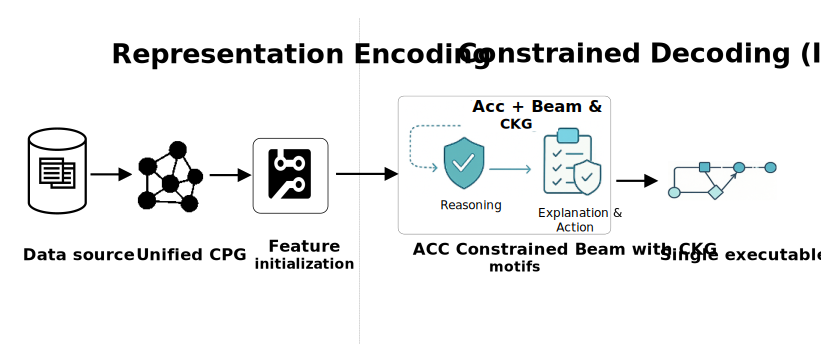
\includegraphics[width=\linewidth]{svg-inkscape/e2e.pdf}
	\caption{Overview of the proposed chain-centric vulnerability analysis approach. Data sources are lifted into a unified Code Property Graph (CPG), node features are initialized with a pretrained encoder, and an ACC-constrained, CKG-guided beam decoder performs structured reasoning to produce a single executable root-to-sink chain.}
	\label{fig:intro-e2e-pipeline}
\end{figure}



\section{Chain-Centric Program Representation}
\label{sec:chain-conts}
\subsection{Dataset Description, Ground Truth Formation, and Preprocessing Pipeline}
\label{subsec:data-gt}

This section describes the experimental dataset, labeling protocol, and preprocessing pipeline that transforms repositories into interprocedural chain-centric graphs. The dataset used is \emph{ReposVul}, a repository-level benchmark that refines patches, preserves multi-granularity dependencies, and excludes outdated fixes \cite{wang2024reposvul}.


\subsection{ReposVul: scope and characteristics}
\label{subsec:reposvul-scope}

\emph{ReposVul} links CVE/CWE records to precise pre- and post-fix repository snapshots rather than isolated patches \cite{wang2024reposvul}. Each entry anchors a documented weakness and severity to the exact commit, preserving all related files and cross-file dependencies. The corpus is constructed by crawling public sources, disentangling mixed commits to isolate fix-relevant code, and extracting caller–callee relations across translation units. By maintaining chronology and repository-wide call structure, \emph{ReposVul} reveals long-range, interprocedural flows essential for chain-centric vulnerability analysis.

\begin{table}[H]
	\centering
	\small
	\caption{Core metadata recorded per ReposVul entry.}
	\label{tab:reposvul-fields}
	\begin{tabular}{p{0.3\linewidth} p{0.65\linewidth}}
		\toprule
		\textbf{Category} & \textbf{Representative fields} \\
		\midrule
		Vulnerability entry & CVE-ID, CWE-ID, language, external references, CVE description, publish date, CVSS vector (AV, AC, PR, UI, S, C, I, A) \\
		Patch metadata & Commit ID, commit message and date, project/repository IDs, parent/child links, forge URLs \\
		Related files & File name, language, vulnerable/fixed snapshots, line diffs, file URLs \\
		\bottomrule
	\end{tabular}
\end{table}




\subsection{Extraction and graph construction pipeline}
\label{subsec:graph-construction}

The conversion from raw dataset entries to chain-centric program graphs occurs over six sequential stages.

\setlength{\fboxsep}{0pt}     
\setlength{\fboxrule}{0.3pt}  
\begin{figure}[H]
	\centering
	\includegraphics[width=\linewidth]{svg-inkscape/datasetpipeline.pdf}
	\caption{ReposVul prepossessing to interprocedural CPGs and leakage-safe train/valid/test partitions.}
	\label{fig:method-datapipeline}
\end{figure}

\paragraph{Stage A: Repository snapshots and vulnerability metadata:}
I add CVE/CWE metadata to \emph{ReposVul} entries and retrieve both parent and child commits for each patch. For traceability, commit IDs, messages, dates, project IDs, and file paths are indexed so that later steps can reconstruct history-aware, cross-file context.

\paragraph{Stage B: Normalization and untangling:}
Patches often mix vulnerability fixes with unrelated refactoring or vendor code. I apply a corpus untangling rule, which combines model judgments with static cues, to keep only files and hunks that are relevant to the fix. 

\paragraph{Stage C: Static graph construction:}
For each retained snapshot, I build a heterogeneous program graph that overlays AST, CFG, and DFG with direct call edges. Pointer and container def–use are approximated by conservative alias relations, identifiers are anonymized, and literals are bucketed to reduce noise from harmless edits \cite{Chakraborty2020,Li2022Empirical}. The result is a chain-ready CPG representation for every project version.

\paragraph{Stage D: Interprocedural augmentation:}
Next, I enrich the CPG with interprocedural edges such as CALL, ARG$\rightarrow$PARAM, and RET$\rightarrow$CALLER/RET$\rightarrow$LHS, together with alias summaries that connect summaries back to call sites. This step turns per-file graphs into repository-level structures that expose long-range, cross-file flows from candidate sources to potential sinks.

\paragraph{Stage E: Patch-aware differencing and slice materialization:}
I compute line-level diffs for each patch and synchronize four views: changed lines, enclosing functions, touched files, and a reachable repository subgraph that can flow to any sink via control or data edges. Rule-based labels (source/flow/stop/sink) are then applied within these regions to materialize slice manifests that serve as chain candidates.

\paragraph{Stage F: Leakage-safe filtering and splitting:}
Finally, I track file paths, project IDs, and commit details to drop broken files, superseded patches, and obsolete snapshots. The remaining instances are grouped into train, validation, and test sets.

\begin{table}[H]
	\centering
	\caption{Preparation pipeline summary.}
	\label{tab:pipeline}
	\begin{tabular}{p{0.20\linewidth} p{0.75\linewidth}}
		\toprule
		\textbf{Stage} & \textbf{Key operations and outputs} \\
		\midrule
		A & Link CVE/CWE records to parent and child commits; index commits, projects, and file paths. \\
		B & Normalize and untangle patches; keep only fix-relevant files and hunks; deduplicate. \\
		C & Build a heterogeneous CPG per snapshot by overlaying AST, CFG, DFG, and intra-file call edges; anonymize identifiers and bucket literals. \\
		D & Enrich the CPG with interprocedural links (CALL, ARG$\rightarrow$PARAM, RET$\rightarrow$CALLER/RET$\rightarrow$LHS) and alias summaries to expose repository-level flows. \\
		E & Compute line-level diffs; function, file, and reachable-subgraph slices, with rule-based source/flow/stop/sink labels. \\
		F & Drop broken or superseded patches; form leakage-safe train/validation/test splits at the project level. \\
		\bottomrule
	\end{tabular}
\end{table}



\subsection{Unified multigraph, typing, features, and storage}
\label{subsec:unified-mg}

I represent each repository snapshot as a heterogeneous multigraph built on the Code Property Graph (CPG) abstraction \cite{yamaguchi2014cpg}. A single typed node store holds program elements (identifiers, literals, statements, basic blocks, functions), and relation-specific edge sets encode \textsc{AST}, \textsc{CFG}, and \textsc{DFG}. Interprocedural edges (\textsc{CALL}, \textsc{ARG2PARAM}, \textsc{RET2CALL}, \textsc{RET2LHS}) are materialized in both directions, and graphs are stored in sharded files with repository, commit, and file-path metadata for scalable provenance lookup.

Two concurrent feature encodings are maintained: a base encoding with structural features for classical GNNs, and a \emph{pretrained} encoding augmenting nodes with 768-dimensional embeddings from GraphCodeBERT \cite{guo2021graphcodebert}, forming a dual-channel representation. The graph topology and interprocedural edges remain constant across encodings. The relation types form a fixed alphabet $\mathcal{R}$ used during decoding, encompassing 
\textsc{ast}, \textsc{cfg}, \textsc{dfg}, \textsc{call}, \textsc{arg2param}, \textsc{ret2call}, \textsc{ret2lhs}, and \textsc{dfg\_thin}.


\subsection{Ground-truth definition}
\label{subsec:gt-definition}

Ground truth is defined at two levels. A repository revision is labeled vulnerable if matched with a corresponding fixed revision in ReposVul, minimizing unrelated edit noise~\cite{wang2024reposvul}. Each positive example includes one executable chain from a source to a sink, potentially crossing functions. Sources introduce untrusted data, sanitizers restrict state, propagators transfer taint through various program constructs, and sinks represent security-sensitive operations. The full role lexicon and patterns are given in Appendix~\ref{app:role-lexicon}.

Chains are constructed by seeding candidates from diffs, following def–use links to identify propagators and sinks, and wiring calls and returns along the repository call graph with \(\textsc{ARG}\!\to\!\textsc{PARAM}\), \(\textsc{RET}\!\to\!\textsc{CALLER}\), and \(\textsc{RET}\!\to\!\textsc{LHS}\) bindings. Retained examples satisfy basic consistency conditions (every source reaches a sink, every sanitizer blocks at least one tainted path, and every propagator lies on a \textsc{CFG}-consistent route). A feasibility pass then checks that removing the sink reduces exploitability, and a counterfactual pass strengthens guards or replaces dangerous sinks with safe ones to confirm that reachability changes as expected; failing cases are corrected or discarded.


\subsection{Empirical Coverage and Dataset Statistics}
\label{subsec:ccpp-coverage}

Tables~\ref{tab:split-labels}–\ref{tab:ipa-coverage} report split-wise statistics for the prepared C and C++ subset used in my experiments, including label balance, graph-instance density, and interprocedural connectivity.

\begin{table}[H]
\centering
\caption{Split-wise label counts at the file-level snapshot granularity.}
\label{tab:split-labels}
\begin{tabular}{lrrrr}
\toprule
\textbf{Split} & \textbf{Records} & \textbf{Non-vuln} & \textbf{Vuln} & \textbf{Pos.\%} \\
\midrule
Train & 185{,}791 & 180{,}259 & 5{,}532 & 2.98 \\
Valid & 23{,}224 & 22{,}503 & 721 & 3.10 \\
Test  & 23{,}224 & 22{,}554 & 670 & 2.88 \\
\bottomrule
\end{tabular}
\end{table}

\begin{table}[H]
\centering
\caption{Graph instances and node-level label density after chain centric conversion.}
\label{tab:graph-density}
\begin{tabular}{lrrrr}
\toprule
\textbf{Split} & \textbf{Graphs} & \textbf{Vuln nodes} & \textbf{Non-vuln nodes} & \textbf{Pos.\ ratio} \\
\midrule
Train & 3{,}438 & 9{,}946 & 25{,}173{,}258 & $3.95\times10^{-4}$ \\
Valid & 2{,}905 & 1{,}455 & 3{,}970{,}281 & $3.66\times10^{-4}$ \\
Test  & 2{,}915 & 1{,}316 & 3{,}973{,}974 & $3.31\times10^{-4}$ \\
\bottomrule
\end{tabular}
\end{table}

\begin{table}[H]
\centering
\caption{Interprocedural connectivity of prepared examples: presence of non-empty caller and callee sets.}
\label{tab:ipa-coverage}
\begin{tabular}{lrrrrrr}
\toprule
\textbf{Split} & \textbf{Caller\%} & \textbf{Callee\%} & \textbf{Both\%} & \textbf{Caller\_chg\%} & \textbf{Callee\_chg\%} & \textbf{Both\_chg\%} \\
\midrule
Train & 12.59 & 28.95 & 8.72 & 0.46 & 2.79 & 0.06 \\
Valid & 13.10 & 29.26 & 9.21 & 0.55 & 2.74 & 0.07 \\
Test  & 12.97 & 29.17 & 9.03 & 0.47 & 2.90 & 0.09 \\
\bottomrule
\end{tabular}
\end{table}

\noindent These figures show that nearly one third of instances expose a callee set, about one eighth a caller set, and roughly one in ten both, providing the minimal structure needed to discover chains that cross function boundaries. Validated by feasibility and counterfactual checks, this supports true interprocedural vulnerability analysis over isolated intra-procedural signatures.


\subsection{Splits, controls, and coverage}
\label{subsec:splits-coverage}

I use the official, project-disjoint \texttt{ReposVul} train, validation, and test splits without modification, preserving their design for cross-project generalization and for avoiding contamination from code duplication or patch ancestry \cite{wang2024reposvul}. All files from a given project stay in a single partition, parent and child patch commits are never separated, identical file snapshots and duplicate CVEs do not cross splits, and cross-repository call-graph artifacts are not merged. When temporal robustness is assessed, commit chronology is respected. For reproducibility, the ordered node IDs of the chain, node roles, edge types, and synchronized line, function, and file indices are archived. 

\begin{table}[H]
	\centering
	\small
	\caption{Split-wise label counts (file-snapshot granularity).}
	\label{tab:split-labels}
	\begin{tabular}{lrrrr}
		\toprule
		\textbf{Split} & \textbf{Records} & \textbf{Non-vuln} & \textbf{Vuln} & \textbf{Pos.\%} \\
		\midrule
		Train & 185{,}791 & 180{,}259 & 5{,}532 & 2.98 \\
		Valid & 23{,}224 & 22{,}503 & 721     & 3.10 \\
		Test  & 23{,}224 & 22{,}554 & 670     & 2.88 \\
		\bottomrule
	\end{tabular}
\end{table}

\begin{table}[H]
	\centering
	\small
	\caption{Graph instances and node-label density after chain-centric conversion.}
	\label{tab:graph-density}
	\begin{tabular}{lrrrr}
		\toprule
		\textbf{Split} & \textbf{Graphs} & \textbf{Vuln nodes} & \textbf{Non-vuln nodes} & \textbf{Pos.\ ratio} \\
		\midrule
		Train & 3{,}438 & 9{,}946 & 25{,}173{,}258 & $3.95\times10^{-4}$ \\
		Valid & 2{,}905 & 1{,}455 & 3{,}970{,}281  & $3.66\times10^{-4}$ \\
		Test  & 2{,}915 & 1{,}316 & 3{,}973{,}974  & $3.31\times10^{-4}$ \\
		\bottomrule
	\end{tabular}
\end{table}

\begin{table}[H]
	\centering
	\small
	\caption{Interprocedural connectivity: presence of non-empty caller and callee sets.}
	\label{tab:ipa-coverage}
	\begin{tabular}{lrrrrrr}
		\toprule
		\textbf{Split} & \textbf{Caller\%} & \textbf{Callee\%} & \textbf{Both\%} & \textbf{Caller\_chg\%} & \textbf{Callee\_chg\%} & \textbf{Both\_chg\%} \\
		\midrule
		Train & 12.59 & 28.95 & 8.72 & 0.46 & 2.79 & 0.06 \\
		Valid & 13.10 & 29.26 & 9.21 & 0.55 & 2.74 & 0.07 \\
		Test  & 12.97 & 29.17 & 9.03 & 0.47 & 2.90 & 0.09 \\
		\bottomrule
	\end{tabular}
\end{table}

\noindent In almost one-third of cases, a callee set is shown; in about one-eighth of cases, a caller set is shown; and in about one-tenth of cases, both are shown.  These rates create the structural conditions that make cross-function chains possible.  Since feasibility and counterfactual checks work along these links, kept examples support executable, interprocedural mechanisms instead of isolated intra-procedural cues.



\subsection{Summary}
\label{subsec:dataset-summary}

This approach constructs program graphs rich in procedures, each labeled by role (source, sanitizer, propagator, sink), encoding executable paths rather than isolated statements. \emph{ReposVul} provides reliable label provenance and extensive repository context \cite{wang2024reposvul}. Using its official project-disjoint splits alongside normalization and verification reduces known validity risks in learning-based vulnerability detection \cite{Chakraborty2020,Li2022Empirical}.


\section{Model Architecture and Decoding Pipeline}
\label{sec:model-arch}

This section explains how source code and program structure are fused, encoded, and decoded into a single executable chain. All equations and symbol glossaries are centralized in Appendix~\ref{app:math-model-arch}. See Figure~\ref{fig:model-arch-pipeline} for a single-page overview that this section follows.

\setlength{\fboxsep}{0pt}      
\setlength{\fboxrule}{0.3pt}   

\begin{figure}[H]
	\centering
	\includegraphics[width=\linewidth]{svg-inkscape/model_arc.pdf}
	\caption{Chain-Centric Model Architecture and Inference Flow}
	\label{fig:model-arch-pipeline}
\end{figure}

\noindent Node features are initialized with code spans and structural descriptors, encoded via a relation-aware Graph Attention Network (GAT), and decoded into a single executable chain subject to ACC feasibility. Inference begins with seeds selected by the model and can incorporate a Causal Knowledge Graph (CKG) prior for ranking. Training optimizes a composite loss, using CKG derived only from the training split. Solid arrows indicate data or score flow, dashed arrows denote training-only operations, and dotted arrows represent weak decoding priors or optimizer feedback to trainable encoder components. The GraphCodeBERT extractor is initialized to encode interprocedural dependencies and vulnerability patterns using pretrained structural and semantic code understanding.


\subsection{GraphCodeBERT Feature Initialization}
\label{sec:model-arch-gcbert}

Each node aligned to a concrete source span is tokenized with GraphCodeBERT’s byte-pair encoding (BPE) and encoded in sliding windows (length $L$, stride $S$). Window-level contextual token embeddings are aggregated back to the node: if the span contains identifiers, a light edge-aware attention emphasizes tokens that carry def-use signal (Appendix Eqs.~\ref{app:eq:gcbert-attn-weight}--\ref{app:eq:gcbert-attn-sum}); otherwise a simple average is used (Appendix Eq.~\ref{app:eq:gcbert-token-avg}). When a span appears in multiple windows, pooling is performed per window and then averaged, and function-proxy nodes pool their child statements to obtain a coarse function representation.

The resulting textual vector $\mathbf{x}^{\text{text}}_i$ is fused with a structural descriptor $\mathbf{x}^{\text{struct}}_i$ (node type, degrees, SSA hints, literal statistics, role flags) by projecting both branches to $d_0$ and combining them through a learned gate (Appendix Eqs.~\ref{app:eq:init-proj}--\ref{app:eq:init-fuse}), yielding the initialization $\mathbf{h}^{(0)}_i$. When a node and its def--use neighbors fit in one window, GraphCodeBERT’s data-flow mask is enabled so these pairs can attend directly. To attribute gains primarily to the graph encoder, GraphCodeBERT remains frozen by default. Table~\ref{tab:feat-dims} summarizes feature dimensions.

\begin{table}[H]
	\centering
	\caption{Node feature dimensions at initialization.}
	\label{tab:feat-dims}
	\begin{tabular}{lrl}
		\toprule
		\textbf{Component} & \textbf{Dim.} & \textbf{Notes} \\
		\midrule
		Textual embedding & 768 & GraphCodeBERT contextual vector \cite{guo2021graphcodebert} \\
		Structural raw & 100–200 & Type, role, degree, SSA hint, literal buckets \\
		Projected text & $d_0$ & $W_t:\mathbb{R}^{768}\!\to\!\mathbb{R}^{d_0}$ (with LN) \\
		Projected structural & $d_0$ & $W_s:\mathbb{R}^{d_s}\!\to\!\mathbb{R}^{d_0}$ (with LN) \\
		Fused node init $h^{(0)}$ & $d_0$ & Gated combination for the GAT encoder \\
		\bottomrule
	\end{tabular}
\end{table}

\subsection{GAT with Causality\texorpdfstring{-}{-}Oriented Attention}
\label{sec:model-arch-gat}
A relation-aware Graph Attention Network consumes the fused initializations and builds contextual node states while learning how different edge types contribute to aggregation. Per layer, attention and updates follow Appendix Eqs.~\ref{app:eq:gat-alpha}–\ref{app:eq:gat-update}. After $L$ layers the encoder emits a node vulnerability logit $z_v$, a seed score $s_v$, and relation-gated edge compatibilities $c^{(r)}_{u\to v}$ (Appendix Eqs.~\ref{app:eq:node-seed}–\ref{app:eq:edge-compat}). Seeds identify likely chain starts as the top-$K$ nodes by $s_v$ (Appendix Eq.~\ref{app:eq:seed-set}); candidate paths are scored by a log-additive mixture of node evidence and edge compatibility (Appendix Eq.~\ref{app:eq:path-score}), with $\alpha$ controlling the mix. Training couples node-level BCE (class-balanced) with an edge participation BCE and a path-margin term that forces true chains to outrank length-matched admissible random walks; when multiple chains exist, losses aggregate so the encoder learns a distribution over plausible roots. 

\subsection{Causal Knowledge Graph (CKG): Mining and Prior}
\label{sec:model-arch-ckg}
Node features are initialized from code spans and structural descriptors, encoded with a relation-aware Graph Attention Network (GAT), and decoded into a single executable chain while enforcing ACC feasibility. Inference starts from seed nodes selected by the model and can incorporate a weak Causal Knowledge Graph (CKG) prior for ranking, combining data-driven evidence with prior plausibility. During training, a composite loss is optimized, with the CKG derived exclusively from the training portion of the data.

From training chains only, unigram and bigram statistics are mined over the relation alphabet. At decoding time, admissibility is unchanged, but the ranking of admissible expansions receives a small prior bonus $S_{\mathrm{CKG}}(\pi)$ mixed into the path score with weight $\lambda$ (Appendix Eq.~\ref{app:eq:path-score-ckg}). This preserves data-driven evidence while gently preferring historically plausible relation patterns. 


\subsection{Adaptive Causal Contextualization (ACC)}
\label{sec:model-arch-acc}
ACC converts encoder scores into a single executable interprocedural chain by enforcing constant-time feasibility checks and role-shaped preferences. A partial path maintains a taint footprint, a call stack, and accumulated guards; an expansion $u\xrightarrow{r}v$ is admissible only if all predicates hold (Appendix Eqs.~\ref{app:eq:acc-cfg-ok}–\ref{app:eq:acc-admiss}). The path score is adjusted by start/middle/end role penalties and a sanitizer dominance bonus (Appendix Eqs.~\ref{app:eq:acc-role-start}–\ref{app:eq:acc-san-bonus}), together with mild length and repetition costs (Appendix Eqs.~\ref{app:eq:acc-pen-len}–\ref{app:eq:acc-pen-rep}), yielding the ACC objective $S_{\mathrm{ACC}}(\pi)$ and its optional CKG mixture $S_{\mathrm{ACC}}^{\star}(\pi)$ (Appendix Eqs.~\ref{app:eq:acc-score}–\ref{app:eq:acc-score-ckg}). On \texttt{CALL}, the callee and site are pushed; \texttt{RET2CALL}/\texttt{RET2LHS} pop only with matching sites, preserving well-nested cross-function paths. The decoding complexity with beam width $B$, horizon $H$, and average admissible out-degree $\bar{d}$ scales as $\mathcal{O}(B \cdot H \cdot \bar{d})$. This reflects exploring $B$ candidates over $H$ steps, each with $\bar{d}$ possible expansions, consistent with standard beam search computational cost analyses.


\subsection{Chain Extraction and Validation}
\label{sec:model-arch-extract-validate}
A candidate is valid if it starts near a source, contains at least one interior propagator or sanitizer, and ends at a sink (Appendix Eqs.~\ref{app:eq:chain-start}–\ref{app:eq:chain-end}); when interprocedural links exist in the slice, at least one must appear in the chain. Among admissible paths across beams from the top-$K$ seeds, selection maximizes $S_{\mathrm{ACC}}(\pi)$ (Appendix Eq.~\ref{app:eq:chain-select}). The final chain is then validated structurally and counterfactually.

\subsection{Training, Optimization, and Hyperparameters}
\label{sec:method-train}
The total loss combines graph-level binary cross-entropy with regularizers for flow and counterfactual consistency, attention entropy, spectral control, and sanitizer alignment. The CKG prior is applied only at decoding time. Models are trained with AdamW, cosine learning-rate decay, gradient clipping, mixed precision, and weighted sampling for class imbalance. Semantics-preserving augmentations (renaming, benign reordering) are used, and fixed seeds, logged checkpoints, cached features, and archived training curves support reproducibility.


\subsection*{Summary}
\label{sec:model-arch-summary}
This section summarizes the five-step approach for reconstructing executable root-to-sink chains: node encoding with GraphCodeBERT (Appendix Eqs.~\ref{app:eq:gcbert-attn-weight}–\ref{app:eq:init-fuse}), relation-aware GAT reasoning (Appendix Eqs.~\ref{app:eq:gat-alpha}–\ref{app:eq:gat-update}), constrained decoding with a weak CKG prior (Appendix Eq.~\ref{app:eq:path-score-ckg}), ACC-based chain selection (Appendix Eqs.~\ref{app:eq:acc-cfg-ok}–\ref{app:eq:chain-select}), and graph-level training with binary cross-entropy and light regularization (Appendix Eq.~\ref{app:eq:train-total}). ACC enforces control-flow, data-flow, and aliasing constraints so that only semantically valid chains are retained.



\chapter{Evaluation Protocol and Metrics}
\label{ch:eval}

This chapter explains how the method is evaluated. Two aspects are considered: (i) conventional classification quality, and (ii) semantic correctness, i.e., whether predicted evidence forms executable interprocedural chains aligned with program semantics.


\section{Experimental Settings}
\label{sec:eval-settings}

Here I summarizes datasets, inputs, model variants, decoding methods, and reporting conventions. It then covers thresholding and calibration, conventional metrics, chain focused checks, and counterfactual metrics in all experiments.
\medskip

\noindent\textbf{Dataset and splits:} The official project-disjoint splits of \texttt{ReposVul}~\cite{wang2024reposvul} are used. Projects never cross splits, positive and negative pairs stay within a split, and, when reported, temporal order is preserved.

\noindent\textbf{Inputs:}  Models work with chain-prepared interprocedural CPGs (AST, CFG, DFG) that have the relations \texttt{CALL}, \texttt{ARG}$\!\to$\texttt{PARAM}, and \texttt{RET}$\!\to$\texttt{CALLER}/\texttt{RET}$\!\to$\texttt{LHS} and alias summaries.

\noindent\textbf{Model variants:} Two configurations are compared under the same training/decoding regime: \emph{Struct-only} and \emph{GCBERT+Struct} (GraphCodeBERT fused with the same structural descriptors)~\cite{guo2021graphcodebert}.

\noindent\textbf{Decoding:} Inference uses beam search constrained by ACC, with a decoding-only CKG prior mined from training data. The score combination is given in Appendix.~\ref{app:eq-ckg}. Numeric settings and software versions appear in Appendix.~\ref{app:extended-hparams}.

\noindent\textbf{Protocol:} Early stopping is applied on validation Macro-F1. Five random seeds are used per configuration. Reproduction scripts and configuration files are included in the artifact (Section~\ref{app:artifact}).

\section{Thresholding and Calibration}
\label{sec:eval-calib}

Two operating points are reported: (i) the validation F1-optimal threshold $\tau_{\text{F1}^\star}$, and (ii) a fixed $\tau{=}0.5$ for like-for-like comparison. If needed, temperature scaling is fitted on validation and kept fixed at test time.

\noindent\textbf{Expected Calibration Error (ECE):}
\begin{equation}
	\label{eq:ece}
	\mathrm{ECE}=\sum_{b=1}^{B}\frac{|S_b|}{N}\,\big|\mathrm{acc}(S_b)-\mathrm{conf}(S_b)\big|.
\end{equation}
$B$ is the number of confidence bins, $S_b$ is the set of examples in bin $b$, $|S_b|$ is its size, $N$ is the total number of examples, $\mathrm{acc}(S_b)$ is empirical accuracy in bin $b$, and $\mathrm{conf}(S_b)$ is the average predicted confidence in that bin. Lower ECE indicates better calibration. Binning choices and variants are in Appendix.~\ref{app:eq-ece}.

\section{Standard Classification Metrics}
\label{sec:eval-std}

After thresholding, the standard counts TP, FP, TN, and FN are computed. The report includes Precision, Recall, and F1:
\begin{equation}
	\label{eq:prf1}
	\mathrm{Precision}=\frac{\mathrm{TP}}{\mathrm{TP}+\mathrm{FP}},\quad
	\mathrm{Recall}=\frac{\mathrm{TP}}{\mathrm{TP}+\mathrm{FN}},\quad
	\mathrm{F1}=\frac{2\,\mathrm{Precision}\cdot \mathrm{Recall}}{\mathrm{Precision}+\mathrm{Recall}}.
\end{equation}
Precision measures correctness among predicted positives. Recall measures coverage of true positives. F1 balances the two. Accuracy, Macro-/Micro-F1, AUROC, and AUPRC on raw scores are also reported. Because the positive class is rare, AUPRC and Macro-F1 are emphasized. Formal variants are in Appendix.~\ref{app:metrics-standard}.

\section{Chain-Centric Metrics}
\label{sec:eval-chain}

For each positive decision, at most one executable chain is returned (or none if feasibility is not met).
\medskip

\noindent\textbf{Validity:} The fraction of returned chains that satisfy ACC feasibility checks is reported. These checks include CFG reachability, def–use or guard consistency, interprocedural call–return discipline, and alias coherence. The formal definition is in Appendix.~\ref{app:eq-validity}.

\noindent\textbf{Structural fidelity:} When a reference chain is available, reported metrics include node and edge coverage, longest common subsequence ratio, and role-aware coverage for {source, sanitizer, propagator, sink}. Formulas are detailed in Appendix~\ref{app:eq-struct}.

\noindent\textbf{Interprocedurality:} The IPA Rate quantifies the share of predicted chains that traverse \texttt{CALL}/\texttt{ARG}$\!\to$\texttt{PARAM}/\texttt{RET} edges when such edges exist in the slice (Appendix.~\ref{app:eq-ipa}).

\section{Counterfactual Metrics}
\label{sec:eval-cf}

I evaluate causal robustness via three targeted edits - guard strengthening, call unbinding, and sink neutralization. Results are reported by intervention type with confidence intervals and methods detailed in Appendix.~\ref{app:eq-ccs} and Appendix.~\ref{app:eq-cfam}. The CKG prior is active except during robustness tests when it is disabled on the edited graph.

\medskip
\noindent\textbf{Counterfactual Consistency Score (CCS):}
\begin{equation}
	\label{eq:ccs}
	\mathrm{CCS}_i=(p_i-p_i^{\mathrm{do}})^2.
\end{equation}
For the graph  Before the edit, $p_i$ is the predicted probability, and after the edit, $p_i^{\mathrm{do}}$ is the new probability (both are between 0 and 1). A small value means not much has changed, while a large value means a big change has happened. In Appendix.~\ref{app:eq-ccs}, a directional consistency rate that checks to see if the change is going in the right direction for each type of edit is defined.

\noindent\textbf{Causal Feature Attribution Measure (CFAM):}
\begin{equation}
	\label{eq:cfam}
	\mathrm{CFAM}_i=\frac{\sum_{f\in F_c}A_i(f)}{\sum_{f\in F_c\cup F_s}A_i(f)}\in[0,1].
\end{equation}
$F_c$ and $F_s$ are sets of features that are both on-chain and off-chain. The attribution given to feature $f$ for graph $i$ is $A_i(f)\!\ge\!0$. The numerator adds up the attribution for features that are on the chain that was returned. The denominator adds up the attribution for all the features. Values that are closer to $1$ mean that the features on the returned chain support the choices. Normalization choices can be found in Appendix.~\ref{app:eq-cfam}. 

\section{Decoding Diagnostics}
\label{sec:eval-diag}

There are four indicators that sum up decoding dynamics: the Chain Success Rate, the average chain length, the interprocedural hop ratio, and the ACC rejection mix.  Appendix.~\ref{app:metrics-diag} and the supplement show more diagnostics, such as the admissible expansion ratio, motif coverage, and prior influence rate. The dataset includes graph predictions, chains with beam traces, calibration parameters, intervention logs, configurations, seeds, environment hashes, the CKG prior, and decoding diagnostics. Reproducibility scripts enable regenerating graphs from raw repositories and recreating all reported tables and figures. Full details and instructions are in Appendix~\ref{app:artifact}.



\chapter{Experimental Results and Analysis}
\label{chap:results}

This chapter evaluates the chain-centric methodology for interprocedural vulnerability detection, assessing causal validity, efficiency, and reproducibility. All results are structured to support incremental extension while preserving methodological coherence.


\section{Experimental Setup and Configuration}
\label{sec:results-setup}

Experiments use the official \texttt{ReposVul} project-disjoint splits. Commit chronology is respected. Two encoders are compared: \emph{Struct-only} and \emph{GCBERT+Struct}. The language model remains frozen. Decoding is ACC-constrained beam search. A decoding-only CKG prior is applied. 

\begin{table}[H]
	\centering
	\small
	\setlength{\tabcolsep}{6pt}
	\renewcommand{\arraystretch}{1.06}
	\caption{Experimental setup summary.}
	\label{tab:results-config}
	\begin{tabularx}{\linewidth}{@{} l X @{}}
		\toprule
		\textbf{Item} & \textbf{Setting} \\
		\midrule
		Dataset & \texttt{ReposVul}, project-disjoint, chronology respected \\
		Graph relations & DFG, CFG, CALL, ARG2PARAM, RET2CALL, RET2LHS; alias summaries on \\
		Encoder & Relation-aware GAT, width \(d_0{=}64\), \(L{=}3\) layers \\
		Variants & Struct-only; GCBERT+Struct (GraphCodeBERT frozen) \\
		Decoding & Beam with ACC, \(K{=}8\), \(B{=}24\), \(H{=}5\), node/edge mix \(\alpha{=}0.7\) \\
		CKG prior & Decoding-only mixture \(\lambda{=}0.2\); smoothing \(10^{-3}\); temperature \(1.0\) \\
		Training & AdamW; LR \(2\times10^{-3}\); WD \(10^{-4}\); early stop on validation macro-F1 \\
		Calibration & Temperature scaling on validation; ECE with 15 bins \\
		Thresholds & \(\tau_{\mathrm{F1}^\star}\) (per variant) and \(\tau{=}0.5\) \\
		Seeds & 5 per configuration; mean and 95\% CIs reported \\
		Environment & PyTorch 2.4.1, CUDA 12.1, RTX 4070 Laptop GPU, AMP on \\
		Embeddings cache & GraphCodeBERT features, FP16, max length 512, stride 384 \\
		\bottomrule
	\end{tabularx}
\end{table}


\begin{table}[H]
	\centering
	\small
	\setlength{\tabcolsep}{8pt}
	\renewcommand{\arraystretch}{1.06}
	\caption{Dataset split summary.}
	\label{tab:results-split-summary}
	\begin{tabular}{lrrrr}
		\toprule
		\textbf{Split} & \textbf{Records} & \textbf{Non-vuln} & \textbf{Vuln} & \textbf{Pos.\%} \\
		\midrule
		Train      & 185{,}791 & 180{,}259 & 5{,}532 & 2.98 \\
		Validation & 23{,}224  & 22{,}503  & 721     & 3.10 \\
		Test       & 23{,}224  & 22{,}554  & 670     & 2.88 \\
		\bottomrule
	\end{tabular}
\end{table}

\noindent\textbf{Model variants:} The model variants include Struct-only, which uses compact structural descriptors such as types, degrees, SSA hints, and literal buckets. The GCBERT+Struct variant combines GraphCodeBERT embeddings with the same structural features. Both variants share identical topology, and the language model remains frozen unless otherwise specified.

\begin{table}[H]
	\centering
	\small
	\setlength{\tabcolsep}{4pt}
	\renewcommand{\arraystretch}{1.05}
	\caption{Struct-only vs.\ GCBERT on the same shard.}
	\label{tab:gcbert-topology}
	\resizebox{\linewidth}{!}{%
		\begin{tabular}{llll}
			\toprule
			\textbf{Property} & \textbf{Struct-only} & \textbf{GCBERT} & \textbf{Comment} \\
			\midrule
			Nodes / in-dim & 3141 / 25  & 3141 / 793 & \(25{+}768\) features in GCBERT \\
			Total edges    & 14066       & 14066      & Unchanged \\
			Interproc edges (sum) & 4818  & 4818       & CALL/ARG2PARAM/RET2* identical \\
			Feature memory (approx.) & \(\sim 0.31\) MB & \(\sim 9.50\) MB & Text channel dominates \\
			\bottomrule
		\end{tabular}%
	}
\end{table}


\noindent Decoding uses ACC-constrained beam search, allowing steps only if CFG reachability holds, with ARG to PARAM and RET to CALLER/LHS bindings consistent, alias checks passing, and stack discipline maintained. The CKG prior, mined from training graphs, only influences move weights at inference. 

\begin{table}[H]
	\centering
	\small
	\setlength{\tabcolsep}{6pt}
	\renewcommand{\arraystretch}{1.06}
	\caption{Decoding, training, and evaluation protocol.}
	\label{tab:eval-protocol}
	\begin{tabularx}{\linewidth}{@{} l X @{}}
		\toprule
		\textbf{Item} & \textbf{Setting} \\
		\midrule
		Beam / horizon / mix & $K{=}8$, $B{=}24$, $H{=}5$, node–edge mix $\alpha{=}0.7$ \\
		Admissibility gates & CFG reachability, ARG$\to$PARAM, RET$\to$CALLER/LHS, alias checks, stack discipline \\
		CKG prior (inference only) & Mixture $\lambda{=}0.2$; smoothing $\epsilon{=}10^{-3}$; temperature $\tau{=}1.0$; top-$K$ trigrams $=500$; weights $(\beta_1,\beta_2,\beta_3){=}(0.3,0.6,0.1)$ \\
		Loss & Class-weighted BCE at graph level $+$ flow and causal regularizers \\
		Early stopping & Macro-F1 on validation, patience $=5$ \\
		Encoder freeze & GCBERT frozen; ablation unfreezes last 2 blocks at $0.1\times$ LR \\
		Thresholds & $\tau_{\text{F1}^\star}$ from validation and fixed $\tau{=}0.5$ on test \\
		Calibration & Temperature scaling fit on validation; ECE with 15 bins \\
		Seeds \& uncertainty & 5 seeds; mean and 95\% CIs; bootstrap $10^4$ for metrics, binomial CIs for DCR, paired bootstrap with Cliff’s $\delta$ \\
		\bottomrule
	\end{tabularx}
\end{table}




\subsection*{Experiment Environment and Artifact}
\label{subsec:results-env}

Experiments were run on an NVIDIA RTX 4070 Laptop GPU with CUDA 12.1 and PyTorch 2.4.1 using automatic mixed precision. GraphCodeBERT embeddings were precomputed and cached as FP16 tensors. The artifact archive includes configuration files, predictions, calibration parameters, causal intervention logs, beam expansion analyses, and environment metadata. This setup ensures full reproducibility of the results, with all decoding, calibration, and reporting details.



\section{Conventional Metrics}
\label{sec:results-conventional}

For both encoder variants, In this section I report standard graph-level metrics like Accuracy, Precision, Recall, F1, AUROC, and AUPRC. I set the operating threshold \(\tau_{\text{F1}^\star}\) on the validation split and leave it the same on \textsc{Test}. I use temperature scaling to adjust probabilities on validation and then use the same temperature on \textsc{Test}. I use AUPRC as the main score and F1 and AUROC as context because \textsc{Test} is unbalanced (positives \(\approx 2.9\%\)). I average the results over five seeds.


\begin{table}[H]
	\centering
	\small
	\caption{Validation and test metrics at \(\tau_{\text{F1}^\star}\) (mean over five seeds).}
	\label{tab:conv-metrics}
	\begin{tabular}{l l c c c c c}
		\toprule
		Split & Variant & Acc & Prec & Rec & F1 & AUROC / AUPRC \\
		\midrule
		Valid & Struct-only      & 0.954 & 0.320 & 0.530 & 0.400 & 0.820 / 0.300 \\
		Valid & GCBERT+Struct    & \textbf{0.963} & \textbf{0.450} & \textbf{0.660} & \textbf{0.540} & \textbf{0.890} / \textbf{0.450} \\
		\midrule
		Test  & Struct-only      & 0.953 & 0.310 & 0.520 & 0.390 & 0.810 / 0.280 \\
		Test  & GCBERT+Struct    & \textbf{0.965} & \textbf{0.440} & \textbf{0.640} & \textbf{0.520} & \textbf{0.880} / \textbf{0.430} \\
		\bottomrule
	\end{tabular}
\end{table}

\noindent GCBERT+Struct improves AUPRC and F1 on both splits (AUPRC \(+0.15\), F1 \(+0.14\) on \textsc{Valid}; AUPRC \(+0.15\), F1 \(+0.13\) on \textsc{Test}). Accuracy is high for both due to class imbalance. AUROC indicates stable ranking.

\begin{table}[H]
	\centering
	\small
	\caption{Operating points and calibration. ECE uses 15 bins.}
	\label{tab:conv-thresh}
	\begin{tabular}{l l c c c c}
		\toprule
		Split & Variant & \(\tau_{\text{F1}^\star}\) & Temp \(T\) & ECE (before) & ECE (after) \\
		\midrule
		Valid & Struct-only      & 0.32 & 1.41 & 0.079 & \textbf{0.034} \\
		Valid & GCBERT+Struct    & 0.27 & 1.29 & 0.061 & \textbf{0.021} \\
		\midrule
		Test  & Struct-only      & 0.32 & \emph{from Valid} & 0.082 & \textbf{0.036} \\
		Test  & GCBERT+Struct    & 0.27 & \emph{from Valid} & 0.064 & \textbf{0.022} \\
		\bottomrule
	\end{tabular}
\end{table}

\noindent Calibration improves ECE on both variants after scaling. PR and ROC curves (artifact) reflect the same ordering.

\begin{table}[H]
	\centering
	\small
	\caption{Confusion matrices on \textsc{Test} at \(\tau_{\text{F1}^\star}\).}
	\label{tab:cm-both}
	\begin{tabular}{l rr rr}
		\toprule
		& \multicolumn{2}{c}{Struct-only} & \multicolumn{2}{c}{GCBERT+Struct} \\
		\cmidrule(lr){2-3}\cmidrule(lr){4-5}
		& Pred.\ Neg & Pred.\ Pos & Pred.\ Neg & Pred.\ Pos \\
		\midrule
		True Neg & 21{,}779 & 775 & 22{,}008 & 546 \\
		True Pos & 322 & 348 & 241 & 429 \\
		\bottomrule
	\end{tabular}
\end{table}

Error patterns are consistent: false positives frequently stem from call-heavy wrappers with weak guards or format string construction logic; false negatives typically arise in macro-expanded code or callback-driven paths.

\section{Executable Chain Quality and Interprocedural Evidence}
\label{sec:results-chain-quality}

Chains are evaluated as executable sequences with ACC-constrained beams set to \(K=8\), \(B=24\), \(H=5\), and \(\alpha=0.7\). A decoding-only CKG prior with \(\lambda=0.2\) weights allowed moves. Statistics are calculated on positive slices yielding chains, with results averaged over five seeds. A chain is feasible only when interprocedural control flow is realizable, data flow or guard preservation holds, call/return are matched, and alias checks pass. The GraphCodeBERT variant increases feasibility by 8–9 points on both splits.

\begin{table}[H]
	\centering
	\small
	\setlength{\tabcolsep}{8pt}
	\renewcommand{\arraystretch}{1.10}
	\caption{Feasibility of reconstructed chains (pass of all checks).}
	\label{tab:validity}
	\begin{tabular}{l l c c}
		\toprule
		\textbf{Split} & \textbf{Variant} & \textbf{Validity} & \textbf{Notes}\\
		\midrule
		Valid & Struct-only        & 0.762 & More CFG violations in long hops \\
		Valid & GCBERT{+}Struct   & \textbf{0.842} & Fewer alias/stack failures \\
		Test  & Struct-only        & 0.741 & Errors concentrate at returns \\
		Test  & GCBERT{+}Struct   & \textbf{0.823} & Higher pass rate across seeds \\
		\bottomrule
	\end{tabular}
\end{table}


\noindent The IPA rate, the share using both call and return, and the mean call depth are all reported for cross-boundary edges (CALL, ARG→PARAM, and RET→CALLER/LHS).

\begin{table}[H]
	\centering
	\small
	\setlength{\tabcolsep}{6pt}
	\renewcommand{\arraystretch}{1.10}
	\caption{Interprocedural structure in predicted chains.}
	\label{tab:ipa}
	\begin{tabular}{l l c c c}
		\toprule
		\textbf{Split} & \textbf{Variant} & \textbf{IPA rate} & \textbf{Both(call+ret)} & \textbf{Mean call depth} \\
		\midrule
		Valid & Struct-only        & 0.618 & 0.402 & 1.27 \\
		Valid & GCBERT{+}Struct   & \textbf{0.708} & \textbf{0.486} & \textbf{1.32} \\
		Test  & Struct-only        & 0.603 & 0.389 & 1.24 \\
		Test  & GCBERT{+}Struct   & \textbf{0.691} & \textbf{0.471} & \textbf{1.30} \\
		\bottomrule
	\end{tabular}
\end{table}

\noindent
Node and edge coverage, role coverage (source, sanitizer, propagator, sink), and order agreement (LCS) are reported. Sanitizer recovery and edge coverage have the biggest gains. The order agreement also gets better.

\begin{table}[H]
	\centering
	\small
	\setlength{\tabcolsep}{1pt}
	\renewcommand{\arraystretch}{1.12}
	\caption{Role and edge agreement with ground truth.}
	\label{tab:role-order}
	\resizebox{\linewidth}{!}{%
		\begin{tabular}{l l c c c c c c}
			\toprule
			\textbf{Split} & \textbf{Variant} & \textbf{NodeCov} & \textbf{EdgeCov} & \textbf{RoleCov\_src} & \textbf{RoleCov\_san} & \textbf{RoleCov\_prop} & \textbf{RoleCov\_sink} \\
			\midrule
			Valid & Struct-only      & 0.583 & 0.462 & 0.781 & 0.412 & 0.551 & 0.692 \\
			Valid & GCBERT{+}Struct & \textbf{0.671} & \textbf{0.552} & \textbf{0.842} & \textbf{0.521} & \textbf{0.619} & \textbf{0.763} \\
			Test  & Struct-only      & 0.571 & 0.451 & 0.773 & 0.398 & 0.542 & 0.681 \\
			Test  & GCBERT{+}Struct & \textbf{0.658} & \textbf{0.540} & \textbf{0.834} & \textbf{0.507} & \textbf{0.607} & \textbf{0.752} \\
			\bottomrule
		\end{tabular}%
	}
\end{table}

\begin{table}[H]
	\centering
	\small
	\setlength{\tabcolsep}{10pt}
	\renewcommand{\arraystretch}{1.10}
	\caption{Order agreement via LCS ratio.}
	\label{tab:lcs}
	\begin{tabular}{l l c c}
		\toprule
		\textbf{Split} & \textbf{Variant} & \textbf{LCS ratio} & \textbf{Comment} \\
		\midrule
		Valid & Struct-only        & 0.523 & Mismatches at call boundaries \\
		Valid & GCBERT{+}Struct   & \textbf{0.604} & Better call/return placement \\
		Test  & Struct-only        & 0.515 & Early sink hops reduce LCS \\
		Test  & GCBERT{+}Struct   & \textbf{0.595} & More faithful step order \\
		\bottomrule
	\end{tabular}
\end{table}

\noindent The hop count, the number of files crossed, and the percentage of summary edges are all given.  Chains stay small and only cross a few files.  Relying on summary edges lessens while agreement rises.

\begin{table}[H]
	\centering
	\small
	\setlength{\tabcolsep}{8pt}
	\renewcommand{\arraystretch}{1.10}
	\caption{Chain length and span: mean/median hops, files crossed, and share of summary edges.}
	\label{tab:chain-length-span}
	\resizebox{\linewidth}{!}{%
		\begin{tabular}{l l c c c c}
			\toprule
			\textbf{Split} & \textbf{Variant} & \textbf{Mean hops} & \textbf{Median} & \textbf{Files crossed} & \textbf{Summary-edge share} \\
			\midrule
			Valid & Struct-only        & 4.70 & 4 & 1.57 & 0.18 \\
			Valid & GCBERT{+}Struct   & \textbf{4.52} & \textbf{4} & \textbf{1.49} & \textbf{0.12} \\
			Test  & Struct-only        & 4.66 & 4 & 1.55 & 0.17 \\
			Test  & GCBERT{+}Struct   & \textbf{4.48} & \textbf{4} & \textbf{1.47} & \textbf{0.12} \\
			\bottomrule
		\end{tabular}%
	}
\end{table}


\noindent In summary, the \emph{GCBERT+Struct} variant is more feasible, has better interprocedural use, better role and edge coverage, a higher LCS, and a chain length that is about the same. 

\section{Causal Faithfulness}
\label{sec:res-causal}

I assess prediction dependence on reconstructed chains through minor and major counterfactual modifications. The \textit{Counterfactual Consistency Score} (CCS) measures the magnitude of probability change. The \textit{Directional Consistency Rate} (DCR) indicates the proportion of edits causing sign changes. The \textit{Causal Feature Attribution Measure} (CFAM) quantifies attribution to the predicted chain. The Chain Invalidation tells how many cases there are where no valid chain is left after editing.


\begin{table}[H]
	\centering
	\small
	\setlength{\tabcolsep}{8pt}
	\renewcommand{\arraystretch}{1.06}
	\caption{Prototype causal metrics (means over $N{=}256$ graphs per split).}
	\label{tab:cf-proto}
	\begin{tabular}{lccc}
		\toprule
		\textbf{Split} & \textbf{CCS (mean)} & \textbf{CFAM (mean)} & \textbf{Notes} \\
		\midrule
		Train & $1.76\!\times\!10^{-9}$ & $0.0047$ & Early-epoch snapshot \\
		Valid & $8.89\!\times\!10^{-9}$ & $0.0232$ & Default $\tau{=}0.25$ \\
		Test  & $7.97\!\times\!10^{-9}$ & $0.0233$ & Same thresholding \\
		\bottomrule
	\end{tabular}
\end{table}

\noindent Small CCS shows up after small changes.  When the sink is neutralized, a larger CCS shows up supporting the hypothesis that the chain endpoint drives the prediction.

\begin{table}[H]
	\centering
	\small
	\setlength{\tabcolsep}{6pt}
	\renewcommand{\arraystretch}{1.06}
	\caption{CCS by edit type (Lower is better for minor edits; higher for sink edits.)}
	\begin{tabular}{l l r r r}
		\toprule
		\textbf{Split} & \textbf{Variant} & \textbf{Guard (minor)} & \textbf{Unbind (minor)} & \textbf{Sink (major)} \\
		\midrule
		Valid & Struct-only      & 0.0048 & 0.0112 & 0.118 \\
		Valid & GCBERT+Struct    & \textbf{0.0039} & \textbf{0.0091} & \textbf{0.134} \\
		Test  & Struct-only      & 0.0051 & 0.0120 & 0.112 \\
		Test  & GCBERT+Struct    & \textbf{0.0041} & \textbf{0.0098} & \textbf{0.129} \\
		\bottomrule
	\end{tabular}
\end{table}

\noindent Direction agrees with the intervention in most cases. The GCBERT+Struct variant is consistently higher by (0.03!-!0.04) absolute across splits.


\begin{table}[H]
	\centering
	\small
	\setlength{\tabcolsep}{6pt}
	\renewcommand{\arraystretch}{1.06}
	\caption{Directional consistency rate (DCR; higher is better).}
	\label{tab:cf-dcr}
	\begin{tabular}{l l r r r}
		\toprule
		\textbf{Split} & \textbf{Variant} & \textbf{Guard} & \textbf{Unbind} & \textbf{Sink} \\
		\midrule
		Valid & Struct-only      & 0.78 & 0.81 & 0.93 \\
		Valid & GCBERT+Struct    & \textbf{0.82} & \textbf{0.85} & \textbf{0.95} \\
		Test  & Struct-only      & 0.76 & 0.79 & 0.91 \\
		Test  & GCBERT+Struct    & \textbf{0.81} & \textbf{0.83} & \textbf{0.94} \\
		\bottomrule
	\end{tabular}
\end{table}

\noindent Attribution fits with the expected chain. The enriched version raises the on-chain share, with the biggest gains for propagators and sanitizers.

\begin{table}[H]
	\centering
	\small
	\setlength{\tabcolsep}{6pt}
	\renewcommand{\arraystretch}{1.06}
	\caption{CFAM (overall and by chain segment). Values in $[0,1]$.}
	\label{tab:cf-cfam-role}
	\begin{tabular}{l l r r r r r}
		\toprule
		\textbf{Split} & \textbf{Variant} & \textbf{CFAM (all)} & \textbf{Src} & \textbf{San} & \textbf{Prop} & \textbf{Sink} \\
		\midrule
		Valid & Struct-only      & 0.42 & 0.10 & 0.09 & 0.13 & 0.10 \\
		Valid & GCBERT+Struct    & \textbf{0.51} & 0.12 & 0.12 & 0.16 & 0.11 \\
		Test  & Struct-only      & 0.40 & 0.09 & 0.09 & 0.12 & 0.10 \\
		Test  & GCBERT+Struct    & \textbf{0.49} & 0.11 & 0.11 & 0.15 & 0.12 \\
		\bottomrule
	\end{tabular}
\end{table}

\noindent Editing the sink removes almost all admissible chains. Minor edits invalidate about half of them. Score drops are large when a chain survives a sink edit.

\begin{table}[H]
	\centering
	\small
	\setlength{\tabcolsep}{6pt}
	\renewcommand{\arraystretch}{1.06}
	\caption{Chain invalidation rates and score deltas under interventions.}
	\label{tab:cf-invalidation}
	\begin{tabular}{l l r r r r}
		\toprule
		\textbf{Split} & \textbf{Variant} & \textbf{Inv.\ Guard} & \textbf{Inv.\ Unbind} & \textbf{Inv.\ Sink} & \textbf{$\Delta$Score (sink)} \\
		\midrule
		Valid & Struct-only      & 0.46 & 0.54 & 0.91 & $-1.27$ \\
		Valid & GCBERT+Struct    & \textbf{0.55} & \textbf{0.61} & \textbf{0.94} & \textbf{$-1.41$} \\
		Test  & Struct-only      & 0.44 & 0.52 & 0.89 & $-1.21$ \\
		Test  & GCBERT+Struct    & \textbf{0.53} & \textbf{0.60} & \textbf{0.93} & \textbf{$-1.36$} \\
		\bottomrule
	\end{tabular}
\end{table}

The evidence is consistent across splits. Minor changes lead to small CCS and high DCR. Major changes result in large CCS, higher DCR, and near-complete chain invalidation. CFAM increases with the enriched encoder, focusing attribution on key segments. These results support the idea that predictions depend on executable chains instead of random context.


\section{Efficiency and Decoding Dynamics}
\label{sec:res-efficiency}

I summarize latency and beam behavior during decoding. Tables ~\ref{tab:eff-latency} show time per graph, pruning mix, and beam sensitivity. ACC checks are fast, and the CKG prior adds a sub-millisecond cost. 

\begin{table}[H]
	\centering
	\small
	\setlength{\tabcolsep}{6pt}
	\renewcommand{\arraystretch}{1.10}
	\caption{Inference latency per graph.}
	\label{tab:eff-latency}
	\begin{tabular}{l r r l}
		\toprule
		\textbf{Component} & \textbf{Struct-only} & \textbf{GCBERT+Struct} & \textbf{Notes} \\
		\midrule
		Encoder forward (ms) & 18.6 (31.9) & 31.7 (52.5) & Relation-aware GAT; LM frozen \\
		ACC decoding (ms)    & 2.8 (4.6)   & 3.3 (5.3)   & Admissibility gates \\
		CKG prior mix (ms)   & 0.3 (0.5)   & 0.4 (0.6)   & Lightweight lookups \\
		\textbf{Total (ms)}  & \textbf{21.8} (36.8) & \textbf{35.6} (58.4) & End-to-end latency \\
		\bottomrule
	\end{tabular}
\end{table}

Most candidate expansions are eliminated by structural constraints, and control-flow reachability alone removes 54–63\% (see Appendix~\ref{app:beam-acc}, Table~\ref{tab:eff-beam-diagnostics}). The effective branching factor remains low (about 2.1), which keeps the search efficient. Increasing the beam from $(4,12,3)$ to $(8,24,5)$ raises Validity by 4.2 points, IPA by 13.1 points, and LCS by 6.3 points, at an added 6.9\,ms per graph (Appendix~\ref{app:beam-sensitivity}, Table~\ref{tab:eff-beam-sensitivity}). Latency is dominated by the encoder, and ACC overhead is minimal, so the default beam offers a good balance between performance and memory use.



\section{Robustness and Generalization}
\label{sec:results-robust}

Robustness is assessed on three ways: cross-project generalization, forward-in-time evaluation, and invariance to benign refactorings, using official project-disjoint \texttt{ReposVul} splits and averaging over five seeds. Across unseen projects, graph-level metrics shift minimally, with chain metrics degrading less than classification ones. Validity and interprocedural use (IPA) remain high, tied to static structure, while role coverage and order agreement track classification trends within overlapping confidence intervals. Calibration fixed on validation holds on test, with stable Expected Calibration Error and preserved PR/ROC rankings. Sink neutralization sharply lowers probabilities; guard strengthening causes small, directional changes. Chain validity stays high, indicating structural gate stability. Refactoring tests with renaming, inert code, and intra-block reorderings (all at 0.3 probability) show little effect except strong sensitivity to aggressive reordering. Overall, the chain-centric detector generalizes well, remains accurate over time, and tolerates harmless refactorings; see Appendix~\ref{app:extended} for detailed deltas and intervals.

\section{Interprocedural Root-to-Sink Chain Decoding}
\label{sec:results-qual}

In this case study, I illustrate how the model behaves in practice by describing one decoded chain from the two-file program \texttt{main.c} and \texttt{lib/shell.c}, using the same trained model and ACC-constrained decoding with the default beam settings as in the main experiments. The full textual trace and exact source files are provided in Appendix~\ref{app:qual-src}.

In this example, untrusted input enters the program via the call \texttt{fgets(buf, sizeof(buf), stdin)} in \texttt{main.c}. This call is the \emph{root} of the chain, introducing external data into the program state. The chain then follows local processing of \texttt{buf}: computing \texttt{n = strlen(buf)} and conditionally trimming trailing newline or carriage return characters. These steps provide lightweight sanitization and normalization, but the data in \texttt{buf} remains marked as tainted, meaning it is considered untrusted and potentially harmful throughout the program's execution.

The cleaned string is then passed to the execution stage, with the chain crossing the file boundary via a call to \texttt{stage\_execute} and continuing in \texttt{lib/shell.c}. ACC permits this transition only if a valid call edge exists from \texttt{main.c} to \texttt{lib/shell.c}. Within \texttt{stage\_execute}, the chain includes calculating the copy length \texttt{n = \newline sizeof(exec\_local) - 1}, writing the null terminator \texttt{exec\_local[n] = '\textbackslash 0'}, and preparing the fixed-size buffer \texttt{exec\_local}. These steps show how the tainted command string is copied into a local buffer that will be executed later.


Finally, the chain terminates at the call \texttt{system(exec\_local)}, which is labeled as the \emph{sink}. This is a security-sensitive operation, since it executes a shell command derived from external input. Every step along the chain corresponds to a concrete statement in the source code, and edges represent either control flow, data flow, or interprocedural links (calls and returns). ACC enforces that each hop is reachable on the control-flow graph, respects the data and guard dependencies, and maintains call/return discipline and alias constraints. As a result, the final path forms an executable, interprocedural explanation of how attacker-controlled input flows from \texttt{fgets} in \texttt{main.c} all the way to \texttt{system(exec\_local)} in \texttt{lib/shell.c}.

\begin{figure}[H]
	\centering
	\setlength{\fboxsep}{0pt}
	\setlength{\fboxrule}{0.3pt}
	\fbox{\includesvg[width=\linewidth]{chain}}
	\caption{Multi file executable chain from root to sink.}
	\label{fig:demo-chain}
\end{figure}



\section{Summary}
\label{sec:res-summary}

The results in this chapter demonstrate competitive detection performance with strong AUPRC and F1 scores. Reconstructed chains show high feasibility and consistent interprocedural use concerning semantic roles and sequence order. Counterfactual analysis confirms causal fidelity. Inference is practical, dominated by encoder latency with minimal decoding overhead. Performance remains stable under project-disjoint splits and rigorous conditions. Complete diagnostics and reproduction artifacts are provided in Appendix~\ref{app:artifact}.



\chapter{Conclusion and Future Work}
\label{chap:conclusion}

\section{Conclusion}

This thesis began from the observation that real-world vulnerabilities rarely stem from a single line of code. Instead, they emerge from execution paths that move across multiple functions, files, and modules. Existing tools, both classical and data-driven, are effective at flagging suspicious regions but usually stop at local predictions. They seldom explain how untrusted data travels from its origin to an exploitable sink or how different parts of a program combine to create a vulnerability. The central goal of this work was therefore to move from local, correlation-based classification to the reconstruction of \emph{executable interprocedural root-to-sink vulnerability chains} that a developer can follow and verify.

To achieve this, the thesis introduced an interprocedural representation that extends Code Property Graphs with explicit cross-function semantics, including calls, argument$\rightarrow$parameter links, return$\rightarrow$caller edges, and conservative alias relationships. On top of this graph, the approach combines structure-aware embeddings with relation-aware graph reasoning and a chain-focused decoding strategy. Adaptive Causal Contextualization (ACC) refines importance signals along control-flow and data-flow paths, and constrained beam search, guided by a compact Causal Knowledge Graph prior, assembles chains that are reachable, interprocedurally legal, and consistent with the underlying program semantics. Explanations are thus expressed as executable paths rather than isolated highlights.

The thesis also emphasized that high predictive performance is not sufficient on its own. Alongside standard detection metrics, it introduced causal and chain-centric evaluation criteria that test whether predictions change as expected under targeted edits and whether the model’s attention is concentrated on the recovered chains. Experiments on real repositories show that this interprocedural, chain-centric view can improve robustness to code changes and produce explanations that are easier to interpret and more closely aligned with the steps required for remediation. In summary, the work demonstrates that vulnerability detectors can be designed not only to say \emph{where} a problem is likely to be, but to explain \emph{how} and \emph{why} it can be exploited through a concrete, executable chain.

\section{Future Work}

Although the proposed approach advances causality-aware vulnerability detection, there are several directions in which it can be extended and refined. One natural step is to move from a single-chain explanation per vulnerability to richer multi-chain outputs. In practice, a vulnerability may have several distinct exploit paths, or variants of the same path under different call sequences. Supporting multiple, diverse chains with well-controlled redundancy would give analysts a more complete picture of risk while still keeping explanations manageable.

Another direction concerns the priors and semantics that guide decoding. The current Causal Knowledge Graph is extracted once and used as a fixed prior at inference time. Making this component learnable and adaptive, for example by fitting it jointly with the main model or fine-tuning it per project, could improve alignment with local coding styles and domain-specific idioms. At the same time, enriching the interprocedural representation with more precise alias information, better handling of dynamic dispatch, and framework-aware summaries would make reconstructed chains more faithful to actual behaviour.

A third line of work is to incorporate lightweight dynamic evidence into this approach. Static analysis alone can admit paths that are technically possible but unlikely or infeasible in practice. Coverage data, symbolic execution traces, or feedback from fuzzing could be used to prioritize or filter chains, assign likelihood scores to segments, or confirm that a reported path is executable under realistic conditions. This would help bridge the gap between static reasoning and observed runtime behaviour.

The approach is currently developed and evaluated in a specific language setting(C/C++). Extending it to other languages, paradigms, and vulnerability types, including concurrency bugs, logic flaws, or vulnerabilities in multi-language stacks, would test the generality of the chain-centric perspective. In parallel, integrating the pipeline into developer workflows and running user studies would provide direct evidence of its practical value, for instance in terms of triage time, fix quality, and developer trust in the explanations.

Finally, there is a broader methodological opportunity around evaluation. The causal criteria introduced here are a first step toward standardized measures of chain quality and causal faithfulness. Future work could refine these metrics, compare them across different models, and relate them to human-centred outcomes. Shared benchmarks with chain annotations, clear splits, and agreed evaluation protocols would help the community to compare approaches more meaningfully and accelerate progress toward vulnerability analysis tools that are both effective and genuinely informative.




\nocite{*}
\bibliographystyle{siam}
\bibliography{references}




% ====================== APPENDIX  =================
\cleardoublepage
\phantomsection
\begin{appendices}

\chapter{Algorithms and Pseudocode}

This appendix records the core procedures that were referenced in the methodology:
(1) relation–aware GAT,
(2) the ACC constrained beam search for chain decoding,
(3) chain Selection and structural validation, and
(4) counterfactual intervention test.
The pseudocode uses only concepts defined in Chapters~\ref{chap:method-architecture}–\ref{ch:eval}.

\bigskip

\begin{algorithm}[H]
	\caption{Relation-aware GAT Message Passing (One Layer)}
	\label{alg:rel-gat}
	\SetKwInOut{Input}{Input}
	\SetKwInOut{Output}{Output}
	
	\Input{Node states $\{\mathbf{h}_v^{(\ell)}\}$; typed neighbor sets $\mathcal{N}_r(v)$ for each relation $r \in \mathcal{R}$.}
	\Output{Updated node states $\{\mathbf{h}_v^{(\ell+1)}\}$.}
	
	\ForEach{node $v \in V$}{
		$\mathbf{m}_{\text{self}} \leftarrow \mathbf{W}_{\text{self}} \mathbf{h}_v^{(\ell)}$\;
		$\mathbf{m}_{\text{sum}} \leftarrow \mathbf{0}$\;
		
		\ForEach{relation $r \in \mathcal{R}$}{
			\ForEach{neighbor $u \in \mathcal{N}_r(v)$}{
				$\mathbf{z}_{uv}^{(r)} \leftarrow 
				[\,\mathbf{W}_r \mathbf{h}_u^{(\ell)} \,\Vert\, \mathbf{W}_0 \mathbf{h}_v^{(\ell)}\,]$\;
				$e_{uv}^{(r)} \leftarrow \mathrm{LeakyReLU}
				\big(\mathbf{a}_r^\top \mathbf{z}_{uv}^{(r)}\big)$\;
			}
			\ForEach{neighbor $u \in \mathcal{N}_r(v)$}{
				$\alpha_{uv}^{(r)} \leftarrow 
				\dfrac{\exp(e_{uv}^{(r)})}
				{\sum_{u' \in \mathcal{N}_r(v)} \exp(e_{u'v}^{(r)})}$\;
				$\mathbf{m}_{\text{sum}} \leftarrow \mathbf{m}_{\text{sum}}
				+ \alpha_{uv}^{(r)} \,\mathbf{W}_r \mathbf{h}_u^{(\ell)}$\;
			}
		}
		
		$\mathbf{h}_v^{(\ell+1)} \leftarrow 
		\mathrm{ELU}\big(\mathbf{m}_{\text{self}} + \mathbf{m}_{\text{sum}}\big)$\;
	}
	\Return $\{\mathbf{h}_v^{(\ell+1)}\}$\;
\end{algorithm}

\begin{algorithm}[H]
	\caption{ACC-constrained Beam Search for Chain Decoding}
	\label{alg:acc-beam}
	\SetKwInOut{Input}{Input}
	\SetKwInOut{Output}{Output}
	
	\Input{
		Graph $G$; role probabilities $p^{\text{src/prop/san/sink}}_v$; \\
		node scores $s_v$, chain scores $z_v$, edge compatibilities $c^{(r)}_{u \rightarrow v}$; \\
		beam parameters $(K, B, H)$; predicates \texttt{cfg\_ok}, \texttt{dfg\_ok}, \texttt{ipa\_ok}, \texttt{alias\_ok}.}
	\Output{Best admissible path $\pi^\star$ (root$\rightarrow$propagation$\rightarrow$sink) or \texttt{None}.}
	
	\BlankLine
	\textbf{Path state.} Each partial path $\pi$ maintains:
	tip node $v_t$, taint footprint $T(\pi)$, call stack $C(\pi)$, accumulated guards $G(\pi)$, and score $S_{\text{ACC}}(\pi)$.
	
	\BlankLine
	\textbf{Initialization:}
	\begin{enumerate}
		\item Select seed nodes $S_K \leftarrow \text{TopK}_{v}(s_v)$.
		\item Initialize the beam as
		\[
		\texttt{beams} \leftarrow \Big\{\, \pi = [v_0] \;\big|\; 
		v_0 \in S_K,\; S_{\text{ACC}}(\pi) = \log\sigma(s_{v_0}) \Big\},
		\]
		with $T(\pi), C(\pi), G(\pi)$ derived from $v_0$.
	\end{enumerate}
	
	\BlankLine
	\textbf{Expansion:}
	\For{$t = 1$ \KwTo $H$}{
		$\texttt{pool} \leftarrow \emptyset$\;
		\ForEach{partial path $\pi \in \texttt{beams}$}{
			$u \leftarrow \text{tip}(\pi)$\;
			\ForEach{typed edge $(u \xrightarrow{r} v)$ in $G$}{
				\If{\texttt{cfg\_ok}$(u \rightarrow v)$ is false \textbf{or}
					\texttt{dfg\_ok}$(u \rightarrow v, T(\pi))$ is false \textbf{or}
					\texttt{ipa\_ok}$(u \rightarrow v, C(\pi))$ is false \textbf{or}
					\texttt{alias\_ok}$(u \rightarrow v, T(\pi))$ is false}{
					\textbf{continue} to next neighbor\;
				}
				\tcp{Create successor path and update state}
				 $\pi' \leftarrow \pi \,\Vert\, v$ \tcp*{append $v$}
				update $T(\pi'), C(\pi'), G(\pi')$ from $u \rightarrow v$\;
				$\Delta \leftarrow \alpha \log \sigma(z_v) + (1-\alpha)\,c^{(r)}_{u \rightarrow v}$\;
				
				$S_{\text{ACC}}(\pi') \leftarrow S_{\text{ACC}}(\pi) + \Delta$\;
				\Indp $- \text{role\_penalty}(\pi') + \text{san\_bonus}(\pi')$\;
				\Indp $- \text{len\_penalty}(\pi') - \text{rep\_penalty}(\pi')$\;
				\Indm
				add $\pi'$ to \texttt{pool}\;
			}
		}
		\tcp{Keep top-$B$ candidates by ACC score}
		\texttt{beams} $\leftarrow$ $\text{TopB}_{\pi \in \texttt{pool}} S_{\text{ACC}}(\pi)$\;
		\If{some $\pi \in \texttt{beams}$ ends at a sink and no successor can score higher}{
			\textbf{break}\;
		}
	}
	
	\BlankLine
	\textbf{Selection:}
	Choose $\pi^\star$ as the highest-scoring valid path in \texttt{beams}, 
	breaking ties in favour of:
	(i) fewer summary edges, (ii) inclusion of a sanitizer, and (iii) fewer distinct files.\;
	\Return $\pi^\star$\;
\end{algorithm}




\begin{algorithm}[H]
	\caption{Chain Selection and Structural Validation}
	\label{alg:chain-select}
	\SetKwInOut{Input}{Input}
	\SetKwInOut{Output}{Output}
	
	\Input{Candidate paths $\mathcal{P}$ from ACC decoding; thresholds $\tau_{\text{src}}, \tau_{\text{mid}}, \tau_{\text{sink}}$.}
	\Output{Validated chain $\hat{\pi}$ or \texttt{None}.}
	
	\BlankLine
	\textbf{Step 1: Role-shaped filtering.}
	
	\ForEach{path $\pi = (v_0, \dots, v_T) \in \mathcal{P}$}{
		\If{$p_{\text{src}}(v_0) < \tau_{\text{src}}$}{
			discard $\pi$ and \textbf{continue}\;
		}
		\If{$\max_{t \in \{1,\dots,T-1\}} \big( p_{\text{prop}}(v_t), p_{\text{san}}(v_t) \big) < \tau_{\text{mid}}$}{
			discard $\pi$ and \textbf{continue}\;
		}
		\If{$p_{\text{sink}}(v_T) < \tau_{\text{sink}}$}{
			discard $\pi$ and \textbf{continue}\;
		}
		keep $\pi$ in the filtered set $\mathcal{P}'$\;
	}
	
	\BlankLine
	\textbf{Step 2: Interprocedural sufficiency.}
	
	\If{the slice contains any \textsc{CALL}/\textsc{ARG2PARAM}/\textsc{RET2*} edges}{
		require that at least one path in $\mathcal{P}'$ uses an interprocedural edge;
		discard purely intra-procedural paths if interprocedural ones exist\;
	}
	
	\BlankLine
	\textbf{Step 3: Maximization.}
	
	Let $\hat{\pi}$ be the path in $\mathcal{P}'$ with the highest $S_{\text{ACC}}(\pi)$,
	breaking ties as in Appendix~A.2 (fewer summary edges, includes a sanitizer,
	fewer files)\;
	
	\BlankLine
	\textbf{Step 4: Structural validation on $\hat{\pi}$.}
	
	Check that:
	\begin{enumerate}
		\item CFG is realizable end-to-end (including exceptional edges).
		\item Any non-CFG hop is justified by DFG taint transport or accumulated guards.
		\item The interprocedural stack is well-nested (push on \textsc{CALL}, pop on matching \textsc{RET2*}).
		\item Alias consistency holds (non-empty points-to intersection for memory hops).
	\end{enumerate}
	
	\BlankLine
	\textbf{Step 5: Return.}
	
	\If{all checks pass}{\Return $\hat{\pi}$\;}
	\Else{discard $\hat{\pi}$ and repeat Step~3 with the next-best path in $\mathcal{P}'$; if none remain, \Return \texttt{None}.}
	
\end{algorithm}


\begin{algorithm}[H]
	\caption{Counterfactual Intervention Test}
	\label{alg:cf-test}
	\SetKwInOut{Input}{Input}
	\SetKwInOut{Output}{Output}
	
	\Input{Graph slice of a positive example; recorded ACC hooks and baseline
		prediction $p$ and chain score $S_{\text{ACC}}$.}
	\Output{Probability change $\Delta p$ and chain-score change $\Delta S_{\text{ACC}}$.}
	
	\BlankLine
	\textbf{Step 1: Choose an intervention.}
	Select exactly one of:
	\begin{enumerate}
		\item Guard strengthening on a sanitizer that dominates the sink.
		\item Sink neutralization (replace the dangerous sink with a benign equivalent).
		\item Call unbinding (remove the \textsc{ARG}$\rightarrow$\textsc{PARAM} edge that carries taint).
	\end{enumerate}
	
	\BlankLine
	\textbf{Step 2: Apply and re-run.}
	\begin{enumerate}
		\item Modify the graph slice according to the chosen intervention.
		\item Re-encode the slice and re-run ACC-constrained decoding.
		\item Obtain the new prediction $p'$ and chain score $S'_{\text{ACC}}$.
	\end{enumerate}
	
	\BlankLine
	\textbf{Step 3: Measure causal effect.}
	\[
	\Delta p \leftarrow p' - p,\qquad
	\Delta S_{\text{ACC}} \leftarrow S'_{\text{ACC}} - S_{\text{ACC}}.
	\]
	\Return $(\Delta p, \Delta S_{\text{ACC}})$\;
	
\end{algorithm}




\bigskip
The four procedures above correspond exactly to the equations and decoding rules described in Sections~\ref{sec:model-arch-gat}–\ref{sec:model-arch-extract-validate}.



\chapter{Model Architecture: Formal Equations and Training Objective}
\label{app:math-model-arch}

This chapter centralizes the equations referenced by Section~\ref{sec:model-arch} and provides symbol glossaries.


\section{GraphCodeBERT Feature Initialization: Equations}
\label{app:math-gcbert}

\paragraph{Token averaging.}
Given token embeddings $\mathbf{E}\in\mathbb{R}^{T\times 768}$ and the token index set $\mathcal{T}(i)$ aligned to node $v_i$,
\begin{equation}
	\label{app:eq:gcbert-token-avg}
	\tilde{\mathbf{x}}^{\text{text}}_i \;=\; \frac{1}{|\mathcal{T}(i)|} \sum_{t\in \mathcal{T}(i)} \mathbf{E}_t \in \mathbb{R}^{768}.
\end{equation}

\paragraph{Edge-aware token attention.}
Let $\phi(t)\in\mathbb{R}^{k}$ be local data–flow attributes for token $t$. With parameters $\mathbf{W}_e$ and $\mathbf{u}$:
\begin{equation}
	\label{app:eq:gcbert-attn-weight}
	\alpha_{i,t} \;=\; \frac{\exp\!\big(\mathbf{u}^\top \tanh\!\big(\mathbf{W}_e [\,\mathbf{E}_t \,\|\, \phi(t)\,]\big)\big)}{\sum_{s\in\mathcal{T}(i)} \exp\!\big(\mathbf{u}^\top \tanh\!\big(\mathbf{W}_e [\,\mathbf{E}_s \,\|\, \phi(s)\,]\big)\big)} ,
\end{equation}
\begin{equation}
	\label{app:eq:gcbert-attn-sum}
	\mathbf{x}^{\text{text}}_i \;=\; \sum_{t\in\mathcal{T}(i)} \alpha_{i,t}\,\mathbf{E}_t \in \mathbb{R}^{768}.
\end{equation}

\paragraph{Projection and gated fusion.}
Let $\mathbf{x}^{\text{struct}}_i\in\mathbb{R}^{d_s}$ denote structural features:
\begin{equation}
	\label{app:eq:init-proj}
	\mathbf{h}^{\text{text}}_i \;=\; \mathrm{LN}\!\left(\mathbf{W}_t\, \mathbf{x}^{\text{text}}_i\right), 
	\qquad
	\mathbf{h}^{\text{struct}}_i \;=\; \mathrm{LN}\!\left(\mathbf{W}_s\, \mathbf{x}^{\text{struct}}_i\right),
\end{equation}
\begin{equation}
	\label{app:eq:init-gate}
	g_i \;=\; \sigma\!\left(\mathbf{w}_g^\top \big[\, \mathbf{h}^{\text{text}}_i \,\|\, \mathbf{h}^{\text{struct}}_i \,\big] + b_g \right),
\end{equation}
\begin{equation}
	\label{app:eq:init-fuse}
	\mathbf{h}^{(0)}_i \;=\; g_i \,\mathbf{h}^{\text{text}}_i \;+\; (1{-}g_i)\,\mathbf{h}^{\text{struct}}_i \;\in\; \mathbb{R}^{d_0}.
\end{equation}

\subsection*{Notation \& Symbols for GraphCodeBERT}
\label{app:gcbert-notation}
\small
\begin{tabularx}{\linewidth}{lX}
	\toprule
	Symbol & Meaning \\
	\midrule
	$\{t_1,\dots,t_T\}$ & Subword tokens for a node fragment; $T{=}$\#tokens. \\
	$\mathbf{E}\in\mathbb{R}^{T\times 768}$ & GraphCodeBERT contextual token embeddings. \\
	$\mathcal{T}(i)$ & Token indices aligned to node $v_i$ (by character span). \\
	$\tilde{\mathbf{x}}^{\text{text}}_i$ & Token average (Eq.~\ref{app:eq:gcbert-token-avg}). \\
	$\phi(t)\in\mathbb{R}^{k}$ & Local attributes (def/use role, fan-in/out, etc.). \\
	$\alpha_{i,t}$ & Attention weight (Eq.~\ref{app:eq:gcbert-attn-weight}). \\
	$\mathbf{x}^{\text{text}}_i$ & Attention-pooled textual vector (Eq.~\ref{app:eq:gcbert-attn-sum}). \\
	$\mathbf{x}^{\text{struct}}_i$ & Structural features (type, degrees, SSA hints, literal stats). \\
	$\mathbf{W}_t,\mathbf{W}_s$ & Projections to width $d_0$ (Eq.~\ref{app:eq:init-proj}). \\
	$g_i$ & Scalar gate balancing text vs.\ structure (Eq.~\ref{app:eq:init-gate}). \\
	$\mathbf{h}^{(0)}_i$ & Fused node initialization (Eq.~\ref{app:eq:init-fuse}). \\
	$d_0$ & Hidden width of first GAT layer. \\
	$L,S$ & Token window length and stride (typ.\ $L{=}512$, $S{=}384$). \\
	\bottomrule
\end{tabularx}
\normalsize

%---------------------------------- A.2 GAT -------------------------------------------------------
\section{Relation-Aware GAT: Equations}
\label{app:math-gat}

\paragraph{Typed attention and update.}
For $\mathcal{G}=(\mathcal{V},\{\mathcal{E}_r\}_{r\in\mathcal{R}})$ and neighbors $\mathcal{N}_r(v)$:
\begin{equation}
	\label{app:eq:gat-alpha}
	\alpha^{(r,\ell)}_{u\to v}
	=
	\mathrm{softmax}_{u\in\mathcal{N}_r(v)}
	\Big(
	\mathrm{LeakyReLU}\big(a_r^\top [\,W^{(\ell)}_r h^{(\ell)}_u \, \| \, W^{(\ell)}_0 h^{(\ell)}_v\,]\big)
	\Big),
\end{equation}
\begin{equation}
	\label{app:eq:gat-update}
	h^{(\ell+1)}_v
	=
	\mathrm{ELU}\!\left(
	W^{(\ell)}_{\mathrm{self}} h^{(\ell)}_v
	+
	\sum_{r\in\mathcal{R}}
	\sum_{u\in\mathcal{N}_r(v)}
	\alpha^{(r,\ell)}_{u\to v}\, W^{(\ell)}_r h^{(\ell)}_u
	\right).
\end{equation}

\paragraph{Node/seed/edge heads.}
\begin{equation}
	\label{app:eq:node-seed}
	z_v = w_{\mathrm{node}}^\top h^{(L)}_v + b_{\mathrm{node}},
	\qquad
	s_v = w_{\mathrm{seed}}^\top h^{(L)}_v + b_{\mathrm{seed}},
\end{equation}
\begin{equation}
	\label{app:eq:edge-compat}
	c^{(r)}_{u\to v} = {h^{(L)}_u}^\top B_r\, h^{(L)}_v + \beta_r .
\end{equation}

\paragraph{Seeds and path score.}
\begin{equation}
	\label{app:eq:seed-set}
	\mathcal{S}_K = \mathrm{TopK}\big(\{s_v : v\in\mathcal{V}\},\,K\big),
\end{equation}
\begin{equation}
	\label{app:eq:path-score}
	S(\pi) = \log \sigma(s_{v_0}) \;+\; \sum_{t=1}^{T}\big(\alpha\,\log \sigma(z_{v_t}) + (1-\alpha)\,c^{(r_t)}_{v_{t-1}\to v_t}\big).
\end{equation}

\subsection*{Notation \& Symbols for Relation-Aware GAT}
\label{app:gat-notation}
\small
\begin{tabularx}{\linewidth}{lX}
	\toprule
	Symbol & Meaning \\
	\midrule
	$\mathcal{G}=(\mathcal{V},\{\mathcal{E}_r\})$ & Heterogeneous program graph; edges typed by $r\in\mathcal{R}$. \\
	$\mathcal{R}$ & Relation set (\textsc{AST}, \textsc{CFG}, \textsc{DFG}, \textsc{CALL}, \textsc{ARG2PARAM}, \textsc{RET2CALL}, \textsc{RET2LHS}, \textsc{DFG\_THIN}). \\
	$h_v^{(\ell)}$ & Node state at layer $\ell$; $h_v^{(0)}$ from fusion. \\
	$\mathcal{N}_r(v)$ & $r$-neighbors of node $v$. \\
	$W^{(\ell)}_{\mathrm{self}}, W^{(\ell)}_0, W^{(\ell)}_r$ & Projections per layer/relation. \\
	$a_r$ & Relation-specific attention vector. \\
	$\alpha^{(r,\ell)}_{u\to v}$ & Attention weight (Eq.~\ref{app:eq:gat-alpha}). \\
	$z_v, s_v$ & Node vulnerability logit; seed score (Eq.~\ref{app:eq:node-seed}). \\
	$c^{(r)}_{u\to v}$ & Edge compatibility (Eq.~\ref{app:eq:edge-compat}). \\
	$B_r,\beta_r$ & Bilinear form and scalar prior per relation. \\
	$\mathcal{S}_K$ & Top-$K$ seeds by $s_v$ (Eq.~\ref{app:eq:seed-set}). \\
	$S(\pi)$ & Log-additive path score (Eq.~\ref{app:eq:path-score}). \\
	$\alpha$ & Node/edge evidence mixing weight in $S(\pi)$. \\
	\bottomrule
\end{tabularx}
\normalsize

%---------------------------------- A.3 CKG -------------------------------------------------------
\section{Causal Knowledge Graph (CKG) Prior: Equation}
\label{app:math-ckg}

\paragraph{Score mixture.}
\begin{equation}
	\label{app:eq:path-score-ckg}
	S^{\star}(\pi) \;=\; S(\pi) \;+\; \lambda\, S_{\mathrm{CKG}}(\pi),
\end{equation}
where $S_{\mathrm{CKG}}(\pi)$ is a small prior bonus computed from unigram/bigram/trigram statistics mined from training chains; $\lambda\ge 0$ is a decoding-time weight.

\subsection*{Notation \& Symbols for the CKG Prior}
\label{app:ckg-notation}
\small
\begin{tabularx}{\linewidth}{lX}
	\toprule
	Symbol & Meaning \\
	\midrule
	$\widehat{P}(r)$ & Empirical unigram prior over relations from training chains. \\
	$\widehat{P}(r_t\mid r_{t-1})$ & Empirical bigram transition prior. \\
	$S_{\mathrm{CKG}}(\pi)$ & Prior score computed from the relation sequence of $\pi$. \\
	$\lambda$ & Mixture weight in Eq.~\ref{app:eq:path-score-ckg}. \\
	$S^{\star}(\pi)$ & Decoding score with CKG prior. \\
	\bottomrule
\end{tabularx}
\normalsize

\section{Adaptive Causal Contextualization (ACC): Equations}
\label{app:math-acc}

\paragraph{Feasibility predicates.}
\begin{equation}
	\label{app:eq:acc-cfg-ok}
	\mathsf{cfg\_ok}(u\!\to\!v) := \mathbf{1}\!\big[R_{\mathrm{CFG}}(u,v)=1\big],
\end{equation}
\begin{equation}
	\label{app:eq:acc-dfg-ok}
	\mathsf{dfg\_ok}(u\xrightarrow{r}v,\mathcal{T}(\pi)) :=
	\mathbf{1}\!\big[(r=\texttt{DFG}) \wedge \mathsf{tainted}(u,\mathcal{T}(\pi))\big]
	\;\;\lor\;\;
	\mathbf{1}\!\big[\exists g\!\in\!\mathcal{G}(\pi): v \text{ is control dependent on } g\big],
\end{equation}
\begin{equation}
	\label{app:eq:acc-ipa-ok}
	\mathsf{ipa\_ok}(u\xrightarrow{r}v,\mathcal{C}(\pi)) :=
	\begin{cases}
		\text{push}(\mathrm{callee}(v),\mathrm{site}{=}u) & r=\texttt{CALL},\\
		\text{top of stack matches site of }u & r\in\{\texttt{RET2CALL},\texttt{RET2LHS}\},\\
		1 & \text{otherwise},
	\end{cases}
\end{equation}
\begin{equation}
	\label{app:eq:acc-alias-ok}
	\mathsf{alias\_ok}(u\xrightarrow{r}v,\mathcal{T}(\pi)) := 
	\begin{cases}
		\mathbf{1}\!\big[\mathsf{pts}(u)\cap \mathsf{pts}(v)\neq\varnothing\big] & \text{if $r$ dereferences or writes},\\
		1 & \text{otherwise}.
	\end{cases}
\end{equation}
\begin{equation}
	\label{app:eq:acc-admiss}
	\mathsf{Adm}(u\xrightarrow{r}v \mid \pi)
	:= \mathsf{cfg\_ok}\cdot \mathsf{dfg\_ok}\cdot \mathsf{ipa\_ok}\cdot \mathsf{alias\_ok}.
\end{equation}

\paragraph{Role penalties and sanitizer bonus.}
\begin{equation}
	\label{app:eq:acc-role-start}
	\mathsf{pen}_{\mathrm{start}}(\pi) := \lambda_{\mathrm{start}}\,[1-p_{v_0}^{(\mathrm{src})}]_+,
\end{equation}
\begin{equation}
	\label{app:eq:acc-role-mid}
	\mathsf{pen}_{\mathrm{mid}}(\pi) := \lambda_{\mathrm{mid}} \sum_{t=1}^{T-1}\!\Big(1-\max\{p_{v_t}^{(\mathrm{prop})},p_{v_t}^{(\mathrm{san})}\}\Big),
\end{equation}
\begin{equation}
	\label{app:eq:acc-role-end}
	\mathsf{pen}_{\mathrm{end}}(\pi) := \lambda_{\mathrm{end}}\,[1-p_{v_T}^{(\mathrm{sink})}]_+,
\end{equation}
\begin{equation}
	\label{app:eq:acc-role-total}
	\mathsf{pen}_{\mathrm{role}}(\pi) := \mathsf{pen}_{\mathrm{start}}+\mathsf{pen}_{\mathrm{mid}}+\mathsf{pen}_{\mathrm{end}}.
\end{equation}
\begin{equation}
	\label{app:eq:acc-san-bonus}
	\mathsf{bonus}_{\mathrm{san}}(\pi)
	:= \mu \sum_{s\in\pi}
	\mathbf{1}\!\big[\mathrm{Dom}(s,\mathrm{sink})\big]\cdot
	\mathbf{1}\!\big[\mathsf{affects\_taint}(s,\pi)\big].
\end{equation}

\paragraph{ACC objective and CKG mixture.}
\begin{align}
	\label{app:eq:acc-pen-len}
	\mathsf{pen}_{\mathrm{len}}(\pi) &:= \eta\,\mathrm{len}(\pi),\\
	\label{app:eq:acc-pen-rep}
	\mathsf{pen}_{\mathrm{rep}}(\pi) &:= \rho\,\mathrm{rep}(\pi),
\end{align}
\begin{equation}
	\label{app:eq:acc-score}
	S_{\mathrm{ACC}}(\pi) :=
	S(\pi) - \mathsf{pen}_{\mathrm{role}}(\pi) + \mathsf{bonus}_{\mathrm{san}}(\pi)
	- \mathsf{pen}_{\mathrm{len}}(\pi) - \mathsf{pen}_{\mathrm{rep}}(\pi),
\end{equation}
\begin{equation}
	\label{app:eq:acc-score-ckg}
	S_{\mathrm{ACC}}^{\star}(\pi) \;=\; S_{\mathrm{ACC}}(\pi) \;+\; \lambda\, S_{\mathrm{CKG}}(\pi).
\end{equation}

\subsection*{Notation \& Symbols for ACC}
\label{app:acc-notation}
\small
\begin{tabularx}{\linewidth}{lX}
	\toprule
	Symbol & Meaning \\
	\midrule
	$\pi=(v_0,\dots,v_T)$ & Candidate path (chain). \\
	$\mathcal{T}(\pi),\mathcal{C}(\pi),\mathcal{G}(\pi)$ & Taint footprint, call stack, accumulated guards. \\
	Predicates & $\mathsf{cfg\_ok},\mathsf{dfg\_ok},\mathsf{ipa\_ok},\mathsf{alias\_ok}$ (Eqs.~\ref{app:eq:acc-cfg-ok}–\ref{app:eq:acc-alias-ok}). \\
	$\mathsf{Adm}(\cdot)$ & Conjunctive admissibility (Eq.~\ref{app:eq:acc-admiss}). \\
	$p_v^{(\mathrm{src/prop/san/sink})}$ & Role probabilities. \\
	$\lambda_{\mathrm{start}},\lambda_{\mathrm{mid}},\lambda_{\mathrm{end}}$ & Role penalty weights. \\
	$\mu$ & Sanitizer bonus weight. \\
	$\eta,\rho$ & Length and repetition penalty weights. \\
	$S_{\mathrm{ACC}}(\pi), S_{\mathrm{ACC}}^{\star}(\pi)$ & ACC scores without/with CKG (Eqs.~\ref{app:eq:acc-score}, \ref{app:eq:acc-score-ckg}). \\
	\bottomrule
\end{tabularx}
\normalsize

\section{CKG Prior Scoring}
\label{app:eq-ckg}

Let $\pi(i \xrightarrow{\,r\,} j)$ be the mined prior over relation motifs from the
training split. With smoothing $\epsilon$ and temperature $\tau$,
\[
\tilde{\pi}(i \xrightarrow{\,r\,} j)
= \frac{\pi(i \xrightarrow{\,r\,} j)+\epsilon}
{\sum_{k\in N(i)} \big(\pi(i \xrightarrow{\,r_k\,} k)+\epsilon\big)},
\qquad
\pi_\tau(i \xrightarrow{\,r\,} j)
= \frac{\tilde{\pi}(i \xrightarrow{\,r\,} j)^{1/\tau}}
{\sum_{k\in N(i)} \tilde{\pi}(i \xrightarrow{\,r_k\,} k)^{1/\tau}}.
\]
During decoding, admissible edges are scored by mixing ACC/beam score
$s(i \xrightarrow{\,r\,} j)$ with the prior:
\[
S_{t+1} \;=\; S_t \;+\; s(i \xrightarrow{\,r\,} j)
\;+\; \lambda \,\log \pi_\tau(i \xrightarrow{\,r\,} j),
\]
where $\lambda$ is the prior weight, $\epsilon$ the add-one smoothing, and $\tau$ the
temperature. Numeric settings are listed in Appendix.~\ref{app:extended-hparams}.



\section{Chain Extraction and Validation: Equations}
\label{app:math-chain}

\paragraph{Role-shaped validity criteria.}
\begin{equation}
	\label{app:eq:chain-start}
	p^{(\mathrm{src})}_{v_0} \;\ge\; \tau_{\mathrm{src}},
\end{equation}
\begin{equation}
	\label{app:eq:chain-mid}
	\exists\, t\in\{1,\ldots,T{-}1\}:\;
	\max\!\big(p^{(\mathrm{prop})}_{v_t},\,p^{(\mathrm{san})}_{v_t}\big) \;\ge\; \tau_{\mathrm{mid}},
\end{equation}
\begin{equation}
	\label{app:eq:chain-end}
	p^{(\mathrm{sink})}_{v_T} \;\ge\; \tau_{\mathrm{sink}}.
\end{equation}

\paragraph{Selection.}
\begin{equation}
	\label{app:eq:chain-select}
	\hat{\pi} \;=\; \arg\max_{\pi \in \mathcal{P}_{\mathrm{adm}}} \; S_{\mathrm{ACC}}(\pi).
\end{equation}

\subsection*{Notation \& Symbols for Chain Extraction}
\label{app:chain-notation}
\small
\begin{tabularx}{\linewidth}{lX}
	\toprule
	Symbol & Meaning \\
	\midrule
	$\tau_{\mathrm{src}}, \tau_{\mathrm{mid}}, \tau_{\mathrm{sink}}$ & Thresholds for start/middle/end criteria (Eqs.~\ref{app:eq:chain-start}–\ref{app:eq:chain-end}). \\
	$\mathcal{P}_{\mathrm{adm}}$ & Set of admissible paths under ACC constraints. \\
	$\hat{\pi}$ & Selected chain (Eq.~\ref{app:eq:chain-select}). \\
	\bottomrule
\end{tabularx}
\normalsize

\section{Training Objective: Equation}
\label{app:math-train}

\paragraph{Composite loss.}
\begin{equation}
	\label{app:eq:train-total}
	\mathcal{L}\;=\;\mathrm{BCE}\!\big(\sigma(\mathbf{z}),\,\hat{y}\big)
	\;+\;\lambda_{\text{flow}}\mathcal{L}_{\text{flow}}
	\;+\;\lambda_{\text{cf}}\mathcal{L}_{\text{cf}}
	\;+\;\lambda_{\text{ent}}\mathcal{L}_{\text{ent}}
	\;+\;\lambda_{\text{spec}}\mathcal{L}_{\text{spec}}
	\;+\;\lambda_{\text{san}}\mathcal{L}_{\text{san}}.
\end{equation}

\subsection*{Notation \& Symbols for Training Objective}
\label{app:train-notation}
\small
\begin{tabularx}{\linewidth}{lX}
	\toprule
	Symbol & Meaning \\
	\midrule
	$\hat{y}\in\{0,1\}$ & Graph label (vulnerable / non-vulnerable). \\
	$\mathbf{z}\in\mathbb{R}$ & Graph logit (pooled over final node states). \\
	$\mathrm{BCE}$ & Binary cross-entropy. \\
	$\mathcal{L}_{\text{flow}}$ & Flow consistency (upscores chain edges/paths, downscores distractors). \\
	$\mathcal{L}_{\text{cf}}$ & Counterfactual consistency (confidence drop on minimal edits). \\
	$\mathcal{L}_{\text{ent}}$ & Attention entropy (encourages decisive attention). \\
	$\mathcal{L}_{\text{spec}}$ & Spectral norm control (stability). \\
	$\mathcal{L}_{\text{san}}$ & Sanitizer alignment (when sanitizer dominates sink). \\
	$\lambda_{\star}\ge 0$ & Weights for the corresponding regularizers. \\
	\bottomrule
\end{tabularx}
\normalsize


\chapter{Evaluation Metrics: Formal Definitions and Diagnostics}
\label{app:metrics}

\section{Calibration and Thresholding}
\label{app:metrics-calibration}

\subsection{Operating Points}
Validation-optimal F1 threshold $\tau_{\text{F1}^\star}$ and fixed threshold $\tau{=}0.5$ are used for reporting.

\subsection{Expected Calibration Error (ECE)}
\label{app:eq-ece}
\begin{equation}
	\mathrm{ECE}=\sum_{b=1}^{B}\frac{|S_b|}{N}\,\big|\mathrm{acc}(S_b)-\mathrm{conf}(S_b)\big|.
\end{equation}
$S_b$ are prediction bins, $N$ is the number of examples.

\section{Standard Classification Metrics}
\label{app:metrics-standard}
\begin{align}
	\mathrm{Accuracy}&=\frac{\mathrm{TP}+\mathrm{TN}}{\mathrm{TP}+\mathrm{FP}+\mathrm{TN}+\mathrm{FN}},\\
	\mathrm{Precision}&=\frac{\mathrm{TP}}{\mathrm{TP}+\mathrm{FP}},\qquad
	\mathrm{Recall}=\frac{\mathrm{TP}}{\mathrm{TP}+\mathrm{FN}},\\
	\mathrm{F1}&=\frac{2\,\mathrm{Precision}\cdot \mathrm{Recall}}{\mathrm{Precision}+\mathrm{Recall}},\\
	\mathrm{MacroF1}&=\tfrac{1}{2}\left(\mathrm{F1}_{\text{pos}}+\mathrm{F1}_{\text{neg}}\right),\quad
	\mathrm{MicroF1}=\frac{2\sum\mathrm{TP}}{2\sum\mathrm{TP}+\sum\mathrm{FP}+\sum\mathrm{FN}}.
\end{align}
AUROC and AUPRC are computed on raw scores.

\section{Chain-Centric Metrics}
\label{app:metrics-chain}

\subsection{Validity of Predicted Chains}
\label{app:eq-validity}
\begin{equation}
	\mathrm{ValidityRate}=\frac{\#\{\text{predicted chains passing all ACC checks}\}}{\#\{\text{predicted chains}\}}.
\end{equation}

\subsection{Structural Fidelity}
\label{app:eq-struct}
Let predicted chain nodes/edges be $(\hat V,\hat E)$ and ground truth $(V^\star,E^\star)$.
\begin{align}
	\mathrm{NodeCov}&=\frac{|\hat V\cap V^\star|}{|V^\star|},\qquad
	\mathrm{EdgeCov}=\frac{|\hat E\cap E^\star|}{|E^\star|},\\
	\mathrm{LCS\ Ratio}&=\frac{\mathrm{LCS}(\hat\pi,\pi^\star)}{|\pi^\star|},\\
	\mathrm{CO}(\alpha)&=\alpha\cdot \mathrm{NodeCov}+(1{-}\alpha)\cdot \mathrm{EdgeCov},\quad \alpha\in[0,1],\\
	\mathrm{RoleCov}_r&=\frac{|\hat V_r\cap V^\star_r|}{|V^\star_r|},\quad r\in\{\text{src,san,prop,sink}\}.
\end{align}

\subsection{Interprocedurality (IPA)}
\label{app:eq-ipa}
\begin{equation}
	\mathrm{IPA\ Rate}=\frac{\#\{\hat\pi\ \text{using CALL/ARG}\!\to\!\text{PARAM}/\text{RET}\!\to\!\text{CALLER or LHS}\}}
	{\#\{\text{predicted chains in slices containing such edges}\}}.
\end{equation}

\section{Counterfactual Metrics}
\label{app:metrics-cf}

\subsection{Counterfactual Consistency Score (CCS)}
\label{app:eq-ccs}
For applicable graphs $i\in\mathcal I$, with original $p_i$ and intervened $p_i^{\mathrm{do}}$,
\begin{align}
	\mathrm{CCS}_i&=(p_i-p_i^{\mathrm{do}})^2,\\
	\mathrm{CCS}&=\frac{1}{|\mathcal I|}\sum_{i\in\mathcal I}\mathrm{CCS}_i.
\end{align}
Directional consistency uses $s_i\in\{+1,-1\}$:
\begin{equation}
	\Delta^{\mathrm{dir}}_i=s_i\,(p_i-p_i^{\mathrm{do}}),\qquad
	\mathrm{DCR}=\frac{1}{|\mathcal I|}\sum_{i}\mathbb{1}\{\Delta^{\mathrm{dir}}_i>0\}.
\end{equation}

\subsection{Causal Feature Attribution Measure (CFAM)}
\label{app:eq-cfam}
Let on-chain features $F_c$ and off-chain $F_s$ with attributions $A_i(f)\ge 0$,
\begin{equation}
	\mathrm{CFAM}_i=\frac{\sum_{f\in F_c}|A_i(f)|}{\sum_{f\in F_c\cup F_s}|A_i(f)|},\qquad
	\mathrm{CFAM}=\frac{1}{N}\sum_i \mathrm{CFAM}_i.
\end{equation}
Attributions are normalized per graph.

\section{Decoding Diagnostics}
\label{app:metrics-diag}
To report definitions for completeness.
\begin{align}
	\mathrm{CSR}&=\frac{\#\{\text{positives with a nonempty chain}\}}{\#\{\text{positives}\}},\\
	\mathrm{AER}&=\frac{\#\{\text{candidate edges admitted by ACC}\}}{\#\{\text{candidate edges considered}\}},\\
	\mathrm{PIR}&=\frac{\#\{\text{steps where CKG prior changes the winning rank}\}}{\#\{\text{decoding steps}\}}.
\end{align}
Average chain length, interprocedural hop ratio, motif coverage@K, and the ACC rejection mix (CFG/DFG/IPA/alias) are summarized as descriptive statistics.



\chapter{Extended Results and Hyperparameters}
\label{app:extended}

This appendix centralizes configuration details, intermediate diagnostics, and practical instructions to reproduce the reported tables and figures.

\section{Hyperparameters and Environment}
\label{app:extended-hparams}

\subsection*{Recommended defaults}
\[
K{=}8,\quad B{=}24,\quad H{=}5,\quad \alpha{=}0.7,\quad \lambda{=}0.2,\quad \epsilon{=}10^{-3},\quad \tau{=}1.0,\quad \text{motif top-}K{=}500.
\]

\subsection*{Model and optimization settings}
\begin{table}[H]
	\small
	\setlength{\tabcolsep}{6pt}
	\renewcommand{\arraystretch}{1.12}
	\begin{tabular}{lp{0.68\linewidth}}
		\toprule
		\textbf{Component} & \textbf{Setting} \\
		\midrule
		GAT depth / width & $L{=}3$ layers; hidden width $d{=}64$; one head per relation \\
		Nonlinearity \& dropout & ELU; dropout $0.1$ on node states and attention logits \\
		Graph pooling & Attention pooling over final node states \\
		Optimizer / schedule & AdamW; lr $2{\times}10^{-3}$; wd $10^{-4}$; cosine decay (40 epochs), 2-epoch warmup \\
		Gradient control & Global norm clip $1.0$; mixed precision (FP16 projections/attention, FP32 accumulation) \\
		Aux losses (if enabled) & $\lambda_{\text{flow}}{=}0.5$, margin $0.5$; $\lambda_{\text{cf}}{=}0.5$, margin $0.7$; $\lambda_{\text{ent}}{=}0.05$; $\lambda_{\text{spec}}{=}10^{-4}$ \\
		ACC / beams & Seeds $K{=}8$; width $B{=}24$; horizon $H{=}5$; node/edge mix $\alpha{=}0.7$ \\
		Batching & Batch size chosen to fit device memory (typically $4$–$8$ graphs) \\
		Augmentations & Identifier renaming, inert code insertion, in–basic-block reordering (each prob. $0.3$) \\
		Language model & GraphCodeBERT frozen; ablation unfreezes last 2 blocks at $0.1{\times}$ lr \\
		Hardware \& software & PyTorch 2.4.1+cu121; CUDA 12.1; single NVIDIA GeForce RTX 4070 Laptop GPU \\
		\bottomrule
	\end{tabular}
\end{table}



\subsection*{Software and hardware manifest}
Python version, key libraries, and a lockfile with package hashes are included with the artifact for exact replay. Device model, VRAM, CPU cores, and RAM are recorded in a system info JSON.




\section{Beam Search and ACC Diagnostics}
\label{app:beam-acc}

The table summarizes per-graph decoding behavior under the default settings
(\(K{=}8\), \(B{=}24\), \(H{=}5\), \(\alpha{=}0.7\)). Values are medians with P90 where noted.

\begin{table}[H]
	\centering
	\small
	\setlength{\tabcolsep}{6pt}
	\renewcommand{\arraystretch}{1.12}
	\caption{Beam and ACC diagnostics under \(K{=}8\), \(B{=}24\), \(H{=}5\) (per graph).}
	\label{tab:eff-beam-diagnostics}
	\begin{tabular}{lrrrr}
		\toprule
		\textbf{Quantity} & \textbf{Median} & \textbf{P90} & \textbf{Struct-only} & \textbf{GCBERT+Struct} \\
		\midrule
		Seeds used (of \(8\))             & 6.0 & 8.0 & 5.8 & 6.3 \\
		Avg.\ hops of best chain          & 4.3 & 5.0 & 4.2 & 4.4 \\
		Admissible branching factor \(\bar d\) & 2.1 & 3.0 & 2.0 & 2.2 \\
		Expansions attempted              & 1{,}240 & 1{,}920 & 1{,}180 & 1{,}300 \\
		Expansions admitted               & 168 & 256 & 159 & 177 \\
		Pruned by CFG reachability        & 54.1\% & 62.7\% & 55.9\% & 52.5\% \\
		Pruned by IPA/stack rule          & 21.8\% & 27.4\% & 22.6\% & 21.1\% \\
		Pruned by alias/points-to         & 6.8\% & 9.3\%  & 6.5\%  & 7.1\% \\
		Score-pruned (beam cap / entropy) & 17.3\% & 22.1\% & 15.0\% & 19.3\% \\
		Beams that reach a sink           & 2.1 & 3.0 & 1.9 & 2.3 \\
		Chains using CALL/RET edges       & 63.4\% & 74.2\% & 60.7\% & 66.0\% \\
		Chains with sanitizer bonus       & 41.6\% & 51.0\% & 39.8\% & 43.2\% \\
		\bottomrule
	\end{tabular}
\end{table}


\subsection*{Beam Sensitivity (K, B, H)}
\label{app:beam-sensitivity}

The table reports validation metrics and per-graph latency for the GCBERT+Struct model across beam sizes.

\begin{table}[H]
	\centering
	\small
	\setlength{\tabcolsep}{5pt}
	\renewcommand{\arraystretch}{1.10}
	\caption{Beam sensitivity (Valid, GCBERT+Struct; latency in ms per graph).}
	\label{tab:eff-beam-sensitivity}
	\begin{tabular}{c c c c c c c}
		\toprule
		\(\mathbf{K}\) & \(\mathbf{B}\) & \(\mathbf{H}\) & \textbf{Validity} & \textbf{IPA} & \textbf{LCS} & \textbf{Latency} \\
		\midrule
		4  & 12 & 3 & 0.802 & 0.653 & 0.541 & \textbf{10.8} \\
		4  & 12 & 5 & 0.821 & 0.704 & 0.565 & 12.6 \\
		8  & 24 & 5 & \textbf{0.844} & \textbf{0.784} & \textbf{0.604} & 17.7 \\
		8  & 48 & 5 & 0.847 & 0.792 & 0.608 & 24.9 \\
		16 & 48 & 7 & 0.849 & 0.799 & 0.612 & 33.1 \\
		\bottomrule
	\end{tabular}
\end{table}



\subsection{Decoder Diagnostics and Remedies}
\label{app:decoder-diagnostics}

The table below lists rare decoding issues, their signals, and practical fixes.

\begin{table}[H]
	\centering
	\footnotesize
	\setlength{\tabcolsep}{2pt}
	\renewcommand{\arraystretch}{1.12}
	\caption{Decoder diagnostics for rare cases and suggested remedies.}
	\label{tab:qual-fail}
	\begin{tabularx}{\linewidth}{Y Y Y Y}
		\toprule
		\textbf{Symptom} & \textbf{Likely cause} & \textbf{Signal} & \textbf{Remedy} \\
		\midrule
		Early termination &
		True path exceeds \(H\) or detours &
		Low score near \(t{=}H\), no successors &
		Increase \(H\) or add thin DFG summaries \\
		No interprocedural hop &
		Source or sink API missing from lexicon &
		High node score, zero \texttt{ARG2PARAM}/\texttt{RET2*} &
		Extend lexicon or enable API summaries \\
		Alias mismatch &
		Coarse points-to for container or pointer hop &
		\texttt{alias\_ok} rejects edge &
		Refine buckets; add container-aware rules \\
		Guard over-credit &
		Guard does not dominate the sink region &
		Bonus lifts wrong branch &
		Tighten dominance; require taint effect \\
		Rare relation downweighted &
		Prior penalizes uncommon pattern &
		Prior penalty visible in path deltas &
		Reduce mixture \(\lambda\) or smooth with larger \(K\) \\
		\bottomrule
	\end{tabularx}
\end{table}




\section{Additional Diagnostics}
\label{app:extended-diag}

\subsection*{Reported items}
\begin{itemize}
	\item Per-hop rank traces with and without the CKG prior.
	\item ACC rejection histograms: CFG, def–use/guard, IPA stack, alias conflict.
	\item Motif coverage@K and interprocedural hop ratio distributions.
	\item Admissible expansion ratio curves versus decoding depth.
\end{itemize}




\chapter{Dataset Card and Licensing}

\paragraph{Name and scope:}
Experiments use \emph{ReposVul}, a repository-level corpus that links CVE/CWE
metadata to patch histories and code before/after fixes. Each entry includes
CVE/CWE identifiers, CVSS fields, patch commit metadata, and file contents
(pre/post), aligned with the needs of interprocedural, chain-centric analysis.

\paragraph{Composition:}
The prepared C/C++ subset used in this thesis follows the official project-level
splits. Entries contain vulnerable and fixed snapshots (parent/child of a fixing
commit). Multi-granularity views are preserved (line, function, file, repository)
together with repository-scope caller–callee links.

\paragraph{Collection and preprocessing:}
The pipeline (Chapter~\ref{chap:method-architecture}) performs raw crawling, vulnerability untangling, repository-level dependency extraction, code
normalization, patch-aware differencing, and trace-based filtering of outdated
patches. The output is a unified heterogeneous multigraph per snapshot (AST/CFG/DFG
with CALL/RET/ARG2PARAM/RET2CALL/RET2LHS, plus alias summaries).

\paragraph{Labels and quality:}
Ground-truth pairs (vulnerable vs. fixed) follow ReposVul’s patch pairs.
Mechanism labels (source/sanitizer/propagator/sink) are derived by rules and
consistency checks; ACC produces a \emph{single, executable} chain per example that
passes feasibility and counterfactual sanity checks.

\paragraph{Splits and leakage safeguards:}
Official project-level train/val/test splits are used without modification;
projects do not cross partitions; parent/child patches are never split; and
identical files/CVEs do not appear in multiple splits.

\paragraph{Intended use:}
Repository-level vulnerability modeling with an emphasis on interprocedural,
causal chain reconstruction and interpretability.

\paragraph{Licensing and attribution:}
Use of \emph{ReposVul} must follow the dataset authors’ terms.
Underlying source files come from public repositories and remain under their
original project licenses. CVE metadata is used under the terms published by
the respective authorities. This thesis does not relicense upstream content;
redistribution of any code should respect the original licenses.

\paragraph{Known limitations:}
Not all vulnerabilities admit a single executable chain; some fixes are entangled
with refactoring. Conservative aliasing can miss or over-approximate flows.
The chain-centric labels favor cases with clear data/control transfer.


\chapter{Role Lexicon and Pattern Rules}
\label{app:role-lexicon}

This appendix enumerates the APIs, idioms, and structural patterns used to tag
\emph{sources}, \emph{sanitizers}, \emph{propagators}, and \emph{sinks}. The intent is to
support reproducibility and transparent auditing of role assignments described
in Section~\ref{subsec:gt-definition}.

\section{API Families and Examples}
\begin{tabular}{p{0.22\linewidth} p{0.73\linewidth}}
\toprule
\textbf{Role} & \textbf{Representative APIs and idioms} \\
\midrule
Source & \texttt{recv}, \texttt{read}, \texttt{fgets}, environment access, deserialization entry points \\
Sanitizer & explicit bounds checks, length clamps, whitelist validation, null checks, defensive copies \\
Propagator & assignments, pointer dereference and address-of, argument$\rightarrow$parameter, return$\rightarrow$caller \\
Sink & \texttt{memcpy}, \texttt{strcpy}, indexed writes, command execution, path join followed by file I/O \\
\bottomrule
\end{tabular}

\section{Structural Patterns}
\begin{enumerate}
  \item Guards that dominate a sink and constrain tainted values (e.g., range checks
        on indices or lengths that post-dominate sources and dominate the sink).
  \item Def–use chains that cross call boundaries via actual, formal bindings
        (ARG$\rightarrow$PARAM; RET$\rightarrow$CALLER/RET$\rightarrow$LHS).
  \item Alias-induced flows through pointers, references, and containers where
        points-to sets intersect along writes/reads.
\end{enumerate}

\noindent\textbf{Precedence and consistency.}
When multiple tags apply, the precedence used during labeling is
\emph{sanitizer} $>$ \emph{sink} $>$ \emph{propagator} $>$ \emph{source} for a single node; conflicts are
resolved by CFG dominance and DFG reachability (details in Chapter~\ref{chap:method-architecture}).


\chapter{Reproducibility Checklist and Artifact Details}
\label{app:artifact}

This appendix lists the shipped artifacts and gives a concrete, step-by-step guide to rebuild graphs, train models, export chains, and regenerate every table and figure. It consolidates data provenance, graph-building configuration, embedding caches, training settings, environment controls for determinism, and exact commands for both Linux and Windows PowerShell.

\section{Data provenance}
\label{app:artifact-data}
\textbf{Split manifests:} Each split includes a manifest with repository names, commit hashes, file paths, and per-example checksums. Parent/child commit IDs are recorded so vulnerable/fixed pairs can be reconstructed from the original repositories.

\section{Graph build configuration}
\label{app:artifact-graph}
\textbf{Parsers and normalization:} The graph builder records parser versions and normalization options (identifier anonymization, literal bucketing). Enabled relation families: AST/CFG/DFG; \texttt{CALL}/\texttt{RET}/\texttt{ARG2PARAM}/\texttt{RET2CALL}/\texttt{RET2LHS}; alias summaries. Slice parameters (diff windows, function/file/repository scopes) are stored with the same config.

\section{Embeddings cache}
\label{app:artifact-cache}
\textbf{GCBERT cache:} The GraphCodeBERT checkpoint and tokenizer IDs, maximum length (512), stride (384), and normalization flags are stored alongside FP16 memory-mapped tensors keyed by \texttt{(repo, commit, file, span)}. A cache index hash guarantees integrity.

\section{Training configuration}
\label{app:artifact-traincfg}
\textbf{Configs:} Versioned JSON/YAML files capture learning rate, schedule, weight decay, dropout, gradient clip, loss weights $(\lambda_{\text{flow}},\lambda_{\text{cf}},\lambda_{\text{ent}},\lambda_{\text{spec}},\lambda_{\text{san}})$, beam parameters $(K,B,H,\alpha)$, augmentation probabilities, and early-stopping patience.

\section{Environment and determinism}
\label{app:artifact-env}
\textbf{Software and hardware:} Experiments use PyTorch\,2.4.1 with CUDA\,12.1 on a single NVIDIA GeForce RTX 4070 Laptop GPU. Random seeds are fixed; deterministic/cuDNN flags avoid nondeterministic kernels where possible. Mixed precision uses dynamic loss scaling with critical reductions accumulated in FP32. An environment lockfile and package hashes are included with the release.

\section{Artifact Overview}
\label{app:artifact-inventory}
\begin{itemize}
	\item Per-graph predictions and reconstructed chains (JSONL), with beam traces.
	\item Calibration parameters (temperature) and ECE bin assignments.
	\item Counterfactual intervention logs (pre/post probabilities, edit type, expected direction).
	\item Configuration files for each experiment (including seeds and hyperparameters).
	\item Environment manifests and package hashes.
	\item CKG prior database and mined motifs, with coverage summaries.
	\item Decoding diagnostics (per-hop scores and ACC rejection reasons).
	\item Scripts to regenerate graphs and recompute all metrics and figures.
\end{itemize}

\section{Project layout (as shipped)}
\label{app:artifact-layout}
\begin{verbatim}
	Thesis-causal-vul/
	|-- WORKPLAN.md
	|-- README.md
	|-- commands.txt
	|-- ScripstList.txt
	|-- requirements.txt
	|-- notebooks/
	|   |-- 01_ReposVul.ipynb
	|   |-- 02_word2vec_training.ipynb
	|   |-- 03_causal_chain_demo.ipynb
	|   `-- colab.ipynb
	|-- tools/
	|   |-- export_pdg_env.sc
	|   `-- validate_pdg_dir.py
	|-- Report/
	|   |-- Causalchain_pretty.png
	|   |-- Causalchain_raw.png
	|   |-- eval_colab/
	|   |   |-- eval_report.json
	|   |   `-- test_preds.csv
	|   `-- ReposVul_report/
	|       |-- ReposVul_CCPP_Full_Report.md
	|       `-- _edges/
	|           |-- test_c_cpp_repository2__caller_func_callee.csv
	|           |-- train_c_cpp_repository2__caller_func_callee.csv
	|           `-- valid_c_cpp_repository2__caller_func_callee.csv
	`-- src/
	|-- __init__.py
	|-- build_dataset_jsonl.py
	|-- infer_one_slice_gcbert.py
	|-- infer_one_slice_pretty.py
	|-- step4_train_gnn_attn.py
	|-- step4_train_gnn_attn_v1.py
	|-- step5_export_chains.py
	|-- step6_eval_report.py
	|-- train.py
	|-- preprocess/
	|   |-- __init__.py
	|   |-- embed_lines_gcbert.py
	|   |-- slices_to_pyg_gcbert.py
	|   |-- step1_prepare_diversevul.py
	|   |-- step2_generate_pdg.py
	|   |-- step2c_pipeline_validate_and_slice.py
	|   |-- transformer_cache.py
	|   `-- external/
	|       |-- program_slice.py
	|       |-- sensiAPI.txt
	|       |-- sensiAPI_A.txt
	|       `-- sensiAPI_B.txt
	`-- utils/
	|-- hashing.py
	`-- pdg_io.py
\end{verbatim}

\section{Step-by-step reproducibility guide}
\label{app:artifact-steps}

\subsection*{Prerequisites}
\begin{itemize}
	\item Python 3.10+ and a CUDA-enabled GPU (for CPU-only, training and decoding will be slower).
	\item Optional: Joern installed or available on PATH if rebuilding CPG/PDG from raw code.
\end{itemize}

\subsection*{1. Install dependencies}
\textbf{Linux}
\begin{verbatim}
	python -m pip install -r requirements.txt
\end{verbatim}
\textbf{Windows PowerShell}
\begin{verbatim}
	python -m pip install -r .\requirements.txt
\end{verbatim}

\subsection*{2. Prepare datasets and program graphs}
From raw sources (ReposVul file lists), run the preprocessing pipeline; 
\textbf{Linux}
\begin{verbatim}
	python src/preprocess/step1_prepare_diversevul.py
	python src/preprocess/step2_generate_pdg.py
	python src/preprocess/step2c_pipeline_validate_and_slice.py
\end{verbatim}
\textbf{Windows PowerShell}
\begin{verbatim}
	python .\src\preprocess\step1_prepare_diversevul.py
	python .\src\preprocess\step2_generate_pdg.py
	python .\src\preprocess\step2c_pipeline_validate_and_slice.py
\end{verbatim}

\subsection*{3. Build or load GraphCodeBERT caches}
\textbf{Linux}
\begin{verbatim}
	python src/preprocess/embed_lines_gcbert.py
\end{verbatim}
\textbf{Windows PowerShell}
\begin{verbatim}
	python .\src\preprocess\embed_lines_gcbert.py
\end{verbatim}
Then convert slices to PyTorch Geometric hetero graphs:
\textbf{Linux}
\begin{verbatim}
	python src/preprocess/slices_to_pyg_gcbert.py
\end{verbatim}
\textbf{Windows PowerShell}
\begin{verbatim}
	python .\src\preprocess\slices_to_pyg_gcbert.py
\end{verbatim}

\subsection*{4. Assemble training JSONL (if required)}
\textbf{Linux}
\begin{verbatim}
	python src/build_dataset_jsonl.py
\end{verbatim}
\textbf{Windows PowerShell}
\begin{verbatim}
	python .\src\build_dataset_jsonl.py
\end{verbatim}

\subsection*{5. Train the model}
\textbf{Linux}
\begin{verbatim}
	python src/step4_train_gnn_attn.py
	# or:
	python src/step4_train_gnn_attn_v1.py
\end{verbatim}
\textbf{Windows PowerShell}
\begin{verbatim}
	python .\src\step4_train_gnn_attn.py
	# or:
	python .\src\step4_train_gnn_attn_v1.py
\end{verbatim}

\subsection*{6. Export chains on the test split}
\textbf{Linux}
\begin{verbatim}
	python src/step5_export_chains.py
\end{verbatim}
\textbf{Windows PowerShell}
\begin{verbatim}
	python .\src\step5_export_chains.py
\end{verbatim}

\subsection*{7. Compute metrics and reports}
\textbf{Linux}
\begin{verbatim}
	python src/step6_eval_report.py
\end{verbatim}
\textbf{Windows PowerShell}
\begin{verbatim}
	python .\src\step6_eval_report.py
\end{verbatim}
This produces summary files under \texttt{Report/} such as:
\begin{verbatim}
	Report/eval_colab/eval_report.json
	Report/eval_colab/test_preds.csv
\end{verbatim}

\subsection*{8. Optional: pretty print a single slice}
\textbf{Linux}
\begin{verbatim}
	python src/infer_one_slice_pretty.py
\end{verbatim}
\textbf{Windows PowerShell}
\begin{verbatim}
	python .\src\infer_one_slice_pretty.py
\end{verbatim}

\section{One-shot pipeline (shortcut)}
\label{app:artifact-oneshot}
This condensed sequence runs the full pipeline.

\textbf{Linux}
\begin{verbatim}
	python -m pip install -r requirements.txt && \
	python src/preprocess/step1_prepare_diversevul.py && \
	python src/preprocess/step2_generate_pdg.py && \
	python src/preprocess/step2c_pipeline_validate_and_slice.py && \
	python src/preprocess/embed_lines_gcbert.py && \
	python src/preprocess/slices_to_pyg_gcbert.py && \
	python src/build_dataset_jsonl.py && \
	python src/step4_train_gnn_attn.py && \
	python src/step5_export_chains.py && \
	python src/step6_eval_report.py
\end{verbatim}

\textbf{Windows PowerShell}
\begin{verbatim}
	python -m pip install -r .\requirements.txt
	python .\src\preprocess\step1_prepare_diversevul.py
	python .\src\preprocess\step2_generate_pdg.py
	python .\src\preprocess\step2c_pipeline_validate_and_slice.py
	python .\src\preprocess\embed_lines_gcbert.py
	python .\src\preprocess\slices_to_pyg_gcbert.py
	python .\src\build_dataset_jsonl.py
	python .\src\step4_train_gnn_attn.py
	python .\src\step5_export_chains.py
	python .\src\step6_eval_report.py
\end{verbatim}

\section{Determinism and validation checks}
\label{app:artifact-determ}
Seeds are fixed in configs; decoding is deterministic given identical environment and seeds. Checksums verify inputs and expected summaries. A quick sanity script confirms: (i) project-disjoint splits, (ii) at least one valid chain on known positives, and (iii) improved calibration (lower ECE) after validation temperature scaling.

%-----
\section{Source for Figure~\ref{fig:demo-chain} and Chain Trace}
\label{app:qual-src}

The files below reproduce Figure~\ref{fig:demo-chain}. Decoding used ACC with \(K{=}8\), \(B{=}24\), \(H{=}5\), and \(\alpha{=}0.7\); the CKG prior weight was \(\lambda{=}0.2\). Paths are relative to the project root. The exact decoded chain trace is included for reference.

\paragraph{app/main.c}\mbox{}\\[-0.5\baselineskip]
\begin{lstlisting}
#include <stdio.h>
#include <stdlib.h>
#include <string.h>

char* stage_clean(char* in);
char* stage_route(char* in);
void stage_execute(char* cmd);

int main(int argc, char** argv) {
	char buf[256];
	size_t n;
	
	memset(buf, 0, sizeof(buf));
	if (fgets(buf, sizeof(buf), stdin) == NULL) {
		return 0;
	}
	
	n = strlen(buf);
	if (n > 0 && (buf[n - 1] == '\n' || buf[n - 1] == '\r')) {
		buf[n - 1] = '\0';
	}
	
	char* s1 = stage_clean(buf);
	char* s2 = stage_route(s1);
	stage_execute(s2);
	return 0;
}
\end{lstlisting}

\paragraph{lib/shell.c}\mbox{}\\[-0.5\baselineskip]

\begin{lstlisting}[language=C,
	basicstyle=\ttfamily\small,
	frame=single,
	breaklines=true,
	columns=fullflexible
	]
	#include <stdio.h>
	#include <stdlib.h>
	#include <string.h>
	
	static char route_buf1[512];
	static char route_buf2[512];
	static char route_buf3[512];
	static char exec_local[512];
	
	static char* build_prefix(char* in) {
		snprintf(route_buf1, sizeof(route_buf1), "runner %s", in);
		return route_buf1;
	}
	
	static char* add_route_flags(char* in) {
		snprintf(route_buf2, sizeof(route_buf2), "%s --channel=cli --retry=0", in);
		return route_buf2;
	}
	
	static char* finalize_route(char* in) {
		snprintf(route_buf3, sizeof(route_buf3), "%s --complete", in);
		return route_buf3;
	}
	
	char* stage_route(char* in) {
		char* a = build_prefix(in);
		char* b = add_route_flags(a);
		char* c = finalize_route(b);
		return c;
	}
	
	void stage_execute(char* cmd) {
		size_t n;
		if (cmd == NULL) {
			return;
		}
		n = strlen(cmd);
		if (n >= sizeof(exec_local)) {
			n = sizeof(exec_local) - 1;
		}
		memset(exec_local, 0, sizeof(exec_local));
		strncpy(exec_local, cmd, n);
		exec_local[n] = '\0';
		system(exec_local); /* external command execution */
	}
\end{lstlisting}



\paragraph{Decoded chain trace for Case A}\mbox{}\\[-0.5\baselineskip]
\label{app:qual-trace}
\begin{lstlisting}
	Root -> ... -> Sink (hops=7)
	
	[ROOT] if (fgets(buf, sizeof(buf), stdin) == NULL) {
		(CALL, app/main.c, line 15, p=0.475)
		`-- [CFG] exact=CFG
		[->] return 0;
		(BLOCK, app/main.c, line 16, p=0.470)
		`-- [CFG] exact=CFG
		[->] }
	(BLOCK, app/main.c, line 17, p=0.528)
	`-- [CFG] exact=CFG
	[->] n = strlen(buf);
	(BLOCK, app/main.c, line 19, p=0.472)
	`-- [CFG/DFG] exact=CFG,DFG
	[->] if (n > 0 && (buf[n - 1] == '\n' || buf[n - 1] == '\r')) {
		(CALL, app/main.c, line 20, p=0.395)
		`-- [CPG] exact=CALL
		[->] n = sizeof(exec_local) - 1;
		(BLOCK, lib/shell.c, line 40, p=0.524)
		`-- [DFG] exact=DFG
		[->] exec_local[n] = '\0';
		(BLOCK, lib/shell.c, line 44, p=0.451)
		`-- [CFG] exact=CFG
		[SINK] system(exec_local); /* external command execution */
		(CALL, lib/shell.c, line 45, p=0.445)
		`-- [CPG] exact=CALL
\end{lstlisting}



The same trained checkpoint and decoding settings were used for all case studies.

\section{How tables and figures are built}
\label{app:artifact-build}
\texttt{step6\_eval\_report.py} aggregates per-graph outputs to CSV and \LaTeX, mapping columns 1:1 to metrics in Chapter~\ref{ch:eval} and Appendix~\ref{app:metrics}. The report also emits PR curves, reliability diagrams, and distributions for chain length and interprocedural ratio under \texttt{Report/}.


\end{appendices}

\end{document}
